\documentclass[conference,compsoc]{IEEEtran}

% *** CITATION PACKAGES ***
%
\ifCLASSOPTIONcompsoc
  % IEEE Computer Society needs nocompress option
  % requires cite.sty v4.0 or later (November 2003)
  \usepackage[nocompress]{cite}
\else
  % normal IEEE
  \usepackage{cite}
\fi

% *** GRAPHICS RELATED PACKAGES ***
%
\ifCLASSINFOpdf
  % \usepackage[pdftex]{graphicx}
  % declare the path(s) where your graphic files are
  % \graphicspath{{../pdf/}{../jpeg/}}
  % and their extensions so you won't have to specify these with
  % every instance of \includegraphics
  % \DeclareGraphicsExtensions{.pdf,.jpeg,.png}
\else
  % or other class option (dvipsone, dvipdf, if not using dvips). graphicx
  % will default to the driver specified in the system graphics.cfg if no
  % driver is specified.
  % \usepackage[dvips]{graphicx}
  % declare the path(s) where your graphic files are
  % \graphicspath{{../eps/}}
  % and their extensions so you won't have to specify these with
  % every instance of \includegraphics
  % \DeclareGraphicsExtensions{.eps}
\fi

% \pagestyle{plain}

% % Fix for the enumitem package conflict
% \let\labelindent\relax
% \usepackage{enumitem}

% % Fix for the caption package warning
% \usepackage{caption}
% \DeclareCaptionOption{IEEEtran}[]{}

% *** ALIGNMENT PACKAGES ***
%
\usepackage{array}
% Frank Mittelbach's and David Carlisle's array.sty patches and improves
% the standard LaTeX2e array and tabular environments to provide better
% appearance and additional user controls. As the default LaTeX2e table
% generation code is lacking to the point of almost being broken with
% respect to the quality of the end results, all users are strongly
% advised to use an enhanced (at the very least that provided by array.sty)
% set of table tools. array.sty is already installed on most systems. The
% latest version and documentation can be obtained at:
% http://www.ctan.org/pkg/array

% *** PDF, URL AND HYPERLINK PACKAGES ***
%
\usepackage[hyphens]{url}
% url.sty was written by Donald Arseneau. It provides better support for
% handling and breaking URLs. url.sty is already installed on most LaTeX
% systems. The latest version and documentation can be obtained at:
% http://www.ctan.org/pkg/url
% Basically, \url{my_url_here}.

% This template file contains packages and commands that are useful and generic
% across papers.
%
% When adding new commands, you can most likely do that within paper.tex, but
% when adding new packages, you might need to update that here to ensure the
% packages are included in the proper order (a common source of compilation
% errors with LaTeX).

%%%%%%%%%%%%%%%%%%%%%%%%%%%%%%%%%%%%%%%%%%%%%%%%%%%%%%%%%%%%%%%%%%%%%%%%%%%%
% Packages {{{

\usepackage[T1]{fontenc}

\usepackage{color}

% Insert images
\usepackage{graphicx}

% Subfigures.
\usepackage[labelformat=simple]{subcaption}
\usepackage{xspace}
\usepackage{multirow}
\usepackage{makecell} % Not sure if we need this
\usepackage{enumitem} % We do need this for IP Order appendix
%\usepackage[ruled,vlined]{algorithm2e}

\usepackage{ulem}
\normalem

\usepackage{listings}
\lstset{breaklines=true}

\usepackage[export]{adjustbox}
\usepackage{multirow}
\usepackage{booktabs}

\usepackage{algpseudocode}
\usepackage{algorithm}

\usepackage{bigdelim}
\usepackage{changepage}
\usepackage{float}

%%%%%%%%%%%%%%%%%%%%%%%%%%%%%%%%%%%%%%%%%%%%%%%%%%%%%%%%%%%%%%%%%%%%%%%%%%%%
% Only enable this for footnote-style affiliations
%\usepackage{authblk}

% }}}
%%%%%%%%%%%%%%%%%%%%%%%%%%%%%%%%%%%%%%%%%%%%%%%%%%%%%%%%%%%%%%%%%%%%%%%%%%%%
% Commands {{{

\newcommand{\etal}{et~al.\xspace}

\renewcommand\thesubfigure{(\alph{subfigure}) }



% }}}
%%%%%%%%%%%%%%%%%%%%%%%%%%%%%%%%%%%%%%%%%%%%%%%%%%%%%%%%%%%%%%%%%%%%%%%%%%%%
% Environments {{{

\newenvironment{strategy}[1][htb]
  {\renewcommand{\algorithmcfname}{Strategy}
   \begin{algorithm}[#1]%
  }{
   \end{algorithm}
  }

\newenvironment{tightlist}{
	\begin{list}{$\bullet$} {
		\setlength{\itemsep}{0.00cm}
		\setlength{\parskip}{-0.1cm}
	}}{\end{list}}

\newenvironment{widelist}{
	\begin{list}{$\bullet$} {
		\setlength{\leftmargin}{.60cm}
		\setlength{\itemsep}{.00cm}
	}}{\end{list}}

% }}}
%%%%%%%%%%%%%%%%%%%%%%%%%%%%%%%%%%%%%%%%%%%%%%%%%%%%%%%%%%%%%%%%%%%%%%%%%%%%
% Comment Commands {{{

\ifdefined\isFinalized
\newcommand{\NewCommentType}[3]{}
\else
\newcommand{\NewCommentType}[3]{\expandafter\newcommand\csname #1\endcsname[1]{{\color{#2}{#3: ##1}} }}
\fi

% }}}
%%%%%%%%%%%%%%%%%%%%%%%%%%%%%%%%%%%%%%%%%%%%%%%%%%%%%%%%%%%%%%%%%%%%%%%%%%%%
% Line-break nudging {{{

\clubpenalty=10000
\widowpenalty = 10000

\hyphenation{de-a-non-y-mi-za-tion}
\hyphenation{none-the-less}
\hyphenation{libev}
\hyphenation{Shadow-socks}
\hyphenation{Outline-VPN}
\hyphenation{Web-RTC}
\hyphenation{Geo-Lite}
\hyphenation{Ali-ba-ba}
\hyphenation{time-stamp}
\hyphenation{time-stamps}

% }}}
%%%%%%%%%%%%%%%%%%%%%%%%%%%%%%%%%%%%%%%%%%%%%%%%%%%%%%%%%%%%%%%%%%%%%%%%%%%%
% Prettier fonts {{{

\usepackage[override]{cmtt} % make tt font tighter / less ugly

% To render CU tap figure
\usepackage[utf8]{inputenc}
\usepackage{pgfplots}
\DeclareUnicodeCharacter{2212}{−}
\usepgfplotslibrary{groupplots,dateplot}
\usetikzlibrary{patterns,shapes.arrows}
\pgfplotsset{compat=newest}


% }}}
%%%%%%%%%%%%%%%%%%%%%%%%%%%%%%%%%%%%%%%%%%%%%%%%%%%%%%%%%%%%%%%%%%%%%%%%%%%%

%% begin self-added packages

%% % For citations having Chinese characters in the title
\usepackage{CJKutf8}

%%%%%%%%%%%%%%%%%%%%%%%%%%%%%%%%%%%%%%%%%%%%%%%%%%%%%%%%%%%%%%%%%%%%%%%%%%%%

% For tables
\usepackage{multirow}
\usepackage{booktabs}
\usepackage{algpseudocode}
\usepackage{algorithm}
\usepackage{caption}
\usepackage[export]{adjustbox}
\usepackage{siunitx}

%%%%%%%%%%%%%%%%%%%%%%%%%%%%%%%%%%%%%%%%%%%%%%%%%%%%%%%%%%%%%%%%%%%%%%%%%%%%

% Don't use monospace for URLs.
%\urlstyle{same}

%%%%%%%%%%%%%%%%%%%%%%%%%%%%%%%%%%%%%%%%%%%%%%%%%%%%%%%%%%%%%%%%%%%%%%%%%%%%

% To balance references
\usepackage{balance}

%%%%%%%%%%%%%%%%%%%%%%%%%%%%%%%%%%%%%%%%%%%%%%%%%%%%%%%%%%%%%%%%%%%%%%%%%%%%
% Autoref {{{

% Labels for \autoref.
% https://tex.stackexchange.com/a/313508
\def\sectionautorefname{Section}
\def\subsectionautorefname{Section}
\def\algorithmautorefname{Algorithm}

%%%%%%%%%%%%%%%%%%%%%%%%%%%%%%%%%%%%%%%%%%%%%%%%%%%%%%%%%%%%%%%%%%%%%%%%%%%%

%% Parhead
\newcommand{\parhead}[1]{\medskip\Parhead{#1}}
% \Parhead is like \parhead except that it doesn't add preceding vertical space.
\newcommand{\Parhead}[1]{\noindent\textbf{#1}\hskip 0.5em\relax}

%%%%%%%%%%%%%%%%%%%%%%%%%%%%%%%%%%%%%%%%%%%%%%%%%%%%%%%%%%%%%%%%%%%%%%%%%%%%
%% Comments/Notes
%% \newcommand{\todo}[1]{{\color{red}{TODO TK: #1}} }
%% \newcommand{\dml}[1]{{\color{blue}{[[Dave: #1]]}} }
 \newcommand{\note}[1]{{\color{blue}{[[#1]]}} }

%%%%%%%%%%%%%%%%%%%%%%%%%%%%%%%%%%%%%%%%%%%%%%%%%%%%%%%%%%%%%%%%%%%%%%%%%%%%
% Anonymization for CU
\newcommand{\cublong}{University of Colorado Boulder}
%\newcommand{\cublong}{University }
\newcommand{\cub}{CU Boulder}
%\newcommand{\cub}{University }

\newcommand{\Q}[1]{{\color{red}{Question: #1}} }

%%%%%%%%%%%%%%%%%%%%%%%%%%%%%%%%%%%%%%%%%%%%%%%%%%%%%%%%%%%%%%%%%%%%%%%%%%%%
% Disable metadata for reproducible PDF.
% https://tex.stackexchange.com/a/313605
\ifpdf
\pdfinfoomitdate=1
\pdftrailerid{}
\pdfsuppressptexinfo=-1
%\hypersetup{pdfcreator={},pdfproducer={}}
\fi
%%%%%%%%%%%%%%%%%%%%%%%%%%%%%%%%%%%%%%%%%%%%%%%%%%%%%%%%%%%%%%%%%%%%%%%%%%%%
% Suppress page numbers for camera-ready version.
% \pagenumbering{gobble}

%%%%%%%%%%%%%%%%%%%%%%%%%%%%%%%%%%%%%%%%%%%%%%%%%%%%%%%%%%%%%%%%%%%%%%%%%%%%

% Use an unbreakable space before the section number in citations like
% \cite[\S 1.2]{Ref}, rather than the default comma plus breakable space.
\renewcommand{\citemid}{~}

%%%%%%%%%%%%%%%%%%%%%%%%%%%%%%%%%%%%%%%%%%%%%%%%%%%%%%%%%%%%%%%%%%%%%%%%%%%%
% Paper-specific commands {{{

% System name (if applicable)
\newcommand{\name}{$\mathsf{SystemName}$\xspace} % middle of sentence
\newcommand{\Name}{$\mathsf{SystemName}$\xspace} % start of sentence

% Per-author comment commands (they don't appear if you "make finalized")
% 	Colors: black, blue, brown, cyan, darkgray, gray, green, lightgray, lime
% 	magenta, olive, orange, pink, purple, red, teal, violet, white,	yellow
\NewCommentType{todo}{red}{TODO}
\NewCommentType{dml}{violet}{dml}

% }}}
%%%%%%%%%%%%%%%%%%%%%%%%%%%%%%%%%%%%%%%%%%%%%%%%%%%%%%%%%%%%%%%%%%%%%%%%%%%%

% Helpful self-defined command for IEEE author block alignment:
% https://tex.stackexchange.com/questions/458204/ieeetran-document-class-how-to-align-five-authors-properly/458208#458208

\makeatletter
\newcommand{\linebreakand}{%
  \end{@IEEEauthorhalign}
  \hfill\mbox{}\par
  \mbox{}\hfill\begin{@IEEEauthorhalign}
}
\makeatother

% For equal contribution footnote

\makeatletter
\newcommand{\footnotestar}[1]{%
  \begingroup%
  \renewcommand{\thefootnote}{*}%
  \renewcommand{\@makefnmark}{\hbox{\textsuperscript{*}}}%
  \footnotetext{#1}%
  \endgroup%
}
\makeatother


%%%%%%%%%%%%%%%%%%%%%%%%%%%%%%%%%%%%%%%%%%%%%%%%%%%%%%%%%%%%%%%%%%%%%%%%%%%%

% Environment for drawing a sequence of byte-sized boxes around text.
% Use \x for a one-byte box, \xx for a two-byte box, \xxxx for a four-byte box,
% and \xxxxxxxx for an eight-byte box.
% Example:
% \begin{bytebox}
% \x{03}\x{c}\x{o}\x{m}
% \xx{c00c}
% \end{bytebox}

\newlength{\byteboxdim}
\newlength{\byteboxwidth}
% \byteboxpre is empty on entering the bytebox environment. It is overridden in
% \byteboxpost to permit line breaks between cells. No line break is permitted
% before the first cell, in order to keep e.g. opening parentheses attached if adjacent.
\newcommand{\byteboxpre}{}
\newcommand{\byteboxpost}{%
% permit line break before the next cell, if any
\renewcommand{\byteboxpre}{\hspace{0pt}}%
% space backwards for the next cell
\kern-\fboxrule\relax%
\ignorespaces\nopagebreak%
}
\newenvironment{bytebox}{%
\renewcommand{\byteboxpre}{}%
% Size byte cells relative to the size of \strutbox in the current font size.
\setlength{\byteboxdim}{\dimexpr\dp\strutbox + \ht\strutbox}%
\setlength{\byteboxwidth}{\byteboxdim}%
\setlength{\fboxsep}{0pt}%
\ignorespaces%
}{%
\nolinebreak\kern\fboxrule\relax%
}
\newcommand{\x}[2][white]{%
\byteboxpre%
\fcolorbox{frame}{#1}{\makebox[\byteboxwidth]{\rule[-0.2\byteboxdim]{0pt}{0.9\byteboxdim}{\texttt{#2}}}}%
\byteboxpost%
}
\newcommand{\xx}[2][white]{%
\byteboxpre%
\fcolorbox{frame}{#1}{\makebox[\dimexpr 2\byteboxwidth+\fboxrule]{\rule[-0.2\byteboxdim]{0pt}{0.9\byteboxdim}{\texttt{#2}}}}%
% draw tick marks within the box
{%
\color{frame}%
\llap{\rule[-0.2\byteboxdim]{\fboxrule}{0.1\byteboxdim}\hspace{\dimexpr \byteboxwidth+\fboxrule}}%
\llap{\rule[+0.6\byteboxdim]{\fboxrule}{0.1\byteboxdim}\hspace{\dimexpr \byteboxwidth+\fboxrule}}%
}%
\byteboxpost%
}
\newcommand{\xxxx}[2][white]{%
\byteboxpre%
\fcolorbox{frame}{#1}{\makebox[\dimexpr 4\byteboxwidth+3\fboxrule]{\rule[-0.2\byteboxdim]{0pt}{0.9\byteboxdim}{\texttt{#2}}}}%
% draw tick marks within the box
{%
\color{frame}%
\llap{\rule[-0.2\byteboxdim]{\fboxrule}{0.1\byteboxdim}\hspace{\dimexpr 1\byteboxwidth+1\fboxrule}}%
\llap{\rule[-0.2\byteboxdim]{\fboxrule}{0.1\byteboxdim}\hspace{\dimexpr 2\byteboxwidth+2\fboxrule}}%
\llap{\rule[-0.2\byteboxdim]{\fboxrule}{0.1\byteboxdim}\hspace{\dimexpr 3\byteboxwidth+3\fboxrule}}%
\llap{\rule[+0.6\byteboxdim]{\fboxrule}{0.1\byteboxdim}\hspace{\dimexpr 1\byteboxwidth+1\fboxrule}}%
\llap{\rule[+0.6\byteboxdim]{\fboxrule}{0.1\byteboxdim}\hspace{\dimexpr 2\byteboxwidth+2\fboxrule}}%
\llap{\rule[+0.6\byteboxdim]{\fboxrule}{0.1\byteboxdim}\hspace{\dimexpr 3\byteboxwidth+3\fboxrule}}%
}%
\byteboxpost%
}
\newcommand{\xxxxxxxx}[2][white]{%
\byteboxpre%
\fcolorbox{frame}{#1}{\makebox[\dimexpr 8\byteboxwidth+7\fboxrule]{\rule[-0.2\byteboxdim]{0pt}{0.9\byteboxdim}{\texttt{#2}}}}%
% draw tick marks within the box
{%
\color{frame}%
\llap{\rule[-0.2\byteboxdim]{\fboxrule}{0.1\byteboxdim}\hspace{\dimexpr 1\byteboxwidth+1\fboxrule}}%
\llap{\rule[-0.2\byteboxdim]{\fboxrule}{0.1\byteboxdim}\hspace{\dimexpr 2\byteboxwidth+2\fboxrule}}%
\llap{\rule[-0.2\byteboxdim]{\fboxrule}{0.1\byteboxdim}\hspace{\dimexpr 3\byteboxwidth+3\fboxrule}}%
\llap{\rule[-0.2\byteboxdim]{\fboxrule}{0.1\byteboxdim}\hspace{\dimexpr 4\byteboxwidth+4\fboxrule}}%
\llap{\rule[-0.2\byteboxdim]{\fboxrule}{0.1\byteboxdim}\hspace{\dimexpr 5\byteboxwidth+5\fboxrule}}%
\llap{\rule[-0.2\byteboxdim]{\fboxrule}{0.1\byteboxdim}\hspace{\dimexpr 6\byteboxwidth+6\fboxrule}}%
\llap{\rule[-0.2\byteboxdim]{\fboxrule}{0.1\byteboxdim}\hspace{\dimexpr 7\byteboxwidth+7\fboxrule}}%
\llap{\rule[+0.6\byteboxdim]{\fboxrule}{0.1\byteboxdim}\hspace{\dimexpr 1\byteboxwidth+1\fboxrule}}%
\llap{\rule[+0.6\byteboxdim]{\fboxrule}{0.1\byteboxdim}\hspace{\dimexpr 2\byteboxwidth+2\fboxrule}}%
\llap{\rule[+0.6\byteboxdim]{\fboxrule}{0.1\byteboxdim}\hspace{\dimexpr 3\byteboxwidth+3\fboxrule}}%
\llap{\rule[+0.6\byteboxdim]{\fboxrule}{0.1\byteboxdim}\hspace{\dimexpr 4\byteboxwidth+4\fboxrule}}%
\llap{\rule[+0.6\byteboxdim]{\fboxrule}{0.1\byteboxdim}\hspace{\dimexpr 5\byteboxwidth+5\fboxrule}}%
\llap{\rule[+0.6\byteboxdim]{\fboxrule}{0.1\byteboxdim}\hspace{\dimexpr 6\byteboxwidth+6\fboxrule}}%
\llap{\rule[+0.6\byteboxdim]{\fboxrule}{0.1\byteboxdim}\hspace{\dimexpr 7\byteboxwidth+7\fboxrule}}%
}%
\byteboxpost%
}

% Colors available to use as the optional argument to byte \x, \xx, \xxxx.
% Hint: use the online oklch color picker to adjust lightness and chroma and convert back to sRGB.
\definecolor{frame}{gray}{0.40}       % box frame
\definecolor{h} {RGB}{242,242,242} % https://oklch.com/#96,0.000,360,100 header
\definecolor{hc}{RGB}{242,242,242} % https://oklch.com/#96,0.000,360,100 header count fields: QDCOUNT, ANCOUNT, NSCOUNT, ARCOUNT
\definecolor{lp}{RGB}{111,246,253} % https://oklch.com/#90,0.118,200,100 label length prefix
\definecolor{l} {RGB}{204,253,255} % https://oklch.com/#96,0.118,200,100 label byte
\definecolor{q} {RGB}{245,243,224} % https://oklch.com/#96,0.024,100,100 QTYPE, QCLASS
\definecolor{in}{RGB}{252,229,229} % https://oklch.com/#94,0.026,17,100  injected answer resource record
\definecolor{dg}{RGB}{220,254,206} % https://oklch.com/#96,0.072,136,100 "digest" bytes that are the first 4 leaked bytes in some cases
\definecolor{b} {RGB}{247,243,211} % https://oklch.com/#96,0.042,102,100 Wallbleed leaked bytes of memory

%%%%%%%%%%%%%%%%%%%%%%%%%%%%%%%%%%%%%%%%%%%%%%%%%%%%%%%%%%%%%%%%%%%%%%%%%%%%

%% To use \cmark and \xmark
\usepackage{pifont}
\newcommand{\cmark}{\ding{51}}%
\newcommand{\xmark}{\ding{55}}%

%% end self-added packages


\usepackage{hyperref}
\hypersetup{
    colorlinks,
    linkcolor={red!50!black},
    citecolor={blue!50!black},
    urlcolor={blue!80!black}
}
\usepackage{makecell}    % For splitting a cell into multiple lines


% correct bad hyphenation here
\hyphenation{op-tical net-works semi-conduc-tor}


\begin{document}
\title{A Wall Behind A Wall: Emerging Regional Censorship in China}

% author names and affiliations
% use a multiple column layout for up to three different
% affiliations
\author{
  \IEEEauthorblockN{Mingshi Wu\IEEEauthorrefmark{1}}
  \IEEEauthorblockA{GFW Report\\
  gfw.report@protonmail.com}
  \and
  \IEEEauthorblockN{Ali Zohaib\IEEEauthorrefmark{1}}
  \IEEEauthorblockA{University of Massachusetts Amherst\\
  azohaib@umass.edu}
  \linebreakand % <------------- \and with a line-break
  \IEEEauthorblockN{Zakir Durumeric}
  \IEEEauthorblockA{Stanford University\\
  zakir@cs.stanford.edu}
  \and
  \IEEEauthorblockN{Amir Houmansadr}
  \IEEEauthorblockA{University of Massachusetts Amherst\\
  amir@cs.umass.edu}
  \and
  \IEEEauthorblockN{Eric Wustrow}
  \IEEEauthorblockA{University of Colorado Boulder\\
  ewust@colorado.edu}
}
% conference papers do not typically use \thanks and this command
% is locked out in conference mode. If really needed, such as for
% the acknowledgment of grants, issue a \IEEEoverridecommandlockouts
% after \documentclass


% conference papers do not typically use \thanks and this command
% is locked out in conference mode. If really needed, such as for
% the acknowledgment of grants, issue a \IEEEoverridecommandlockouts
% after \documentclass

% for over three affiliations, or if they all won't fit within the width
% of the page (and note that there is less available width in this regard for
% compsoc conferences compared to traditional conferences), use this
% alternative format:
%
%\author{\IEEEauthorblockN{Michael Shell\IEEEauthorrefmark{1},
%Homer Simpson\IEEEauthorrefmark{2},
%James Kirk\IEEEauthorrefmark{3},
%Montgomery Scott\IEEEauthorrefmark{3} and
%Eldon Tyrell\IEEEauthorrefmark{4}}
%\IEEEauthorblockA{\IEEEauthorrefmark{1}School of Electrical and Computer Engineering\\
%Georgia Institute of Technology,
%Atlanta, Georgia 30332--0250\\ Email: see http://www.michaelshell.org/contact.html}
%\IEEEauthorblockA{\IEEEauthorrefmark{2}Twentieth Century Fox, Springfield, USA\\
%Email: homer@thesimpsons.com}
%\IEEEauthorblockA{\IEEEauthorrefmark{3}Starfleet Academy, San Francisco, California 96678-2391\\
%Telephone: (800) 555--1212, Fax: (888) 555--1212}
%\IEEEauthorblockA{\IEEEauthorrefmark{4}Tyrell Inc., 123 Replicant Street, Los Angeles, California 90210--4321}}

% make the title area
\maketitle

\footnotestar{Mingshi Wu and Ali Zohaib contributed equally to this work.}

%%
%% The abstract is a short summary of the work to be presented in the
%% article.
\begin{abstract}

  China has long orchestrated its Internet censorship through relatively
	centralized policies and a unified implementation, known as the Great
	Firewall of China (GFW).  However, since August 2023, anecdotes suggest that
	the Henan Province has deployed its own regional censorship.  In this work,
	we characterize provincial-level censorship in Henan, and compare it with
	the national-level GFW.  We find that Henan has established TLS SNI-based
	and HTTP Host-based censorship that inspects and blocks traffic leaving the
	province.  While the Henan Firewall is less sophisticated and less robust
	against typical network variability, its volatile and aggressive blocking of
	second-level domains made it block ten times more websites than the GFW at
	some points in time.  Based on the observed parsing flaws and injection
	behaviors, we introduce simple client-side methods to bypass censorship in
	the Henan province.  Our work documents an alarming sign of regional
	censorship emerging in China.

\end{abstract}

\section{Introduction}

The People's Republic of China develops and maintains
one of the most sophisticated Internet censorship apparatuses,
colloquially referred to as the Great Firewall (GFW).
Through DNS poisoning~\cite{Duan2012a, Chai2019a, Hoang2021a, Anonymous2020a,Fan2025a},
HTTP Host header filtering~\cite{Clayton2006a, Wang2017a, Rambert2021a, Hoang2024a},
TLS SNI/ESNI filtering~\cite{Chai2019a, Bock2020ESNI, Hoang2024a}~\cite[\S 3]{Bock2021c},
IP address blocking~\cite[\S4]{Chai2019a},
active probing~\cite{Ensafi2015b,Dunna2018a,Alice2020a}~\cite[\S 5]{Wu2023a},
and proxy traffic detection~\cite[\S 4]{Wu2023a},
China blocks its citizens from accessing large swaths of Internet content and services.

China's censorship apparatus has long been believed to be operated relatively centrally,
in terms of both its \textit{policy} and \textit{implementation}.
Empirical measurements have revealed China's %evidences of
uniform and coordinated management of
censorship policies~\cite{Anonymous2020a, Hoang2021a, Wu2023a, Hoang2024a},
software updates~\cite[\S4.5]{Sakamoto2024a}~\cite[\S VII]{Fan2025a},
and infrastructures~\cite[\S3.4]{Alice2020a}~\cite[\S 5]{Anonymous2020a}.
Censorship devices are positioned at the national border~\cite{Xu2011a, Wright2012a, Anonymous2020a},
where they inspect and filter traffic entering or exiting the country.
As a result, traffic exchanged domestically within China is not inspected or blocked by the GFW.

However, recent anecdotes suggest that this centralized and uniform censorship model
may no longer tell the whole story.
In August 2023, users in the Henan Province of China---the third-largest province by
population and a pivotal labor hub---began reporting an uptick in inaccessible
websites that were accessible elsewhere in China~\cite{Henan-user-report}.

In this work,\footnote{Project homepage: \url{https://gfw.report/publications/sp25/en}.}
we first explore a natural question raised by the discovery of
regional censorship in Henan (\autoref{sec:detection}): have other provinces in
China deployed the same or similar regional censorship?  We conducted a
measurement study in seven provinces and municipalities in China, including
Beijing, Shanghai, Guangdong, Zhejiang, Jiangsu, Sichuan, and Henan, to identify
potential regional censorship.
Likely limited by the vantage points we could access in China,
we found no evidence of regional censorship in the six provinces other than Henan.

We then analyze the emerging regional censorship in the Henan Province,
comparing its policies and implementations with the national GFW.
%
As illustrated in~\autoref{fig:two-firewalls}, our investigation reveals that
the provincial-level middleboxes in Henan block access to certain HTTP and HTTPS
websites through both HTTP Host-based and TLS Server Name Indication (SNI)-based
filtering (\autoref{sec:methodology}).  Contrasting the GFW that monitors and
blocks traffic leaving and entering the country, this regional firewall only
censors traffic exiting the province (\autoref{sec:what-targeted}).  It also
differs from the GFW in terms of connection tracking and parsing logic
(\autoref{sec:parsing-logic}), injection behaviors and fingerprints
(\autoref{sec:how-block}), and network location.  (\autoref{sec:location}).
% (which determines the traffic it can inspect and block) and blocklist size and
% update frequency (\autoref{sec:blocklists}).

\begin{figure}[t]
  \centering
  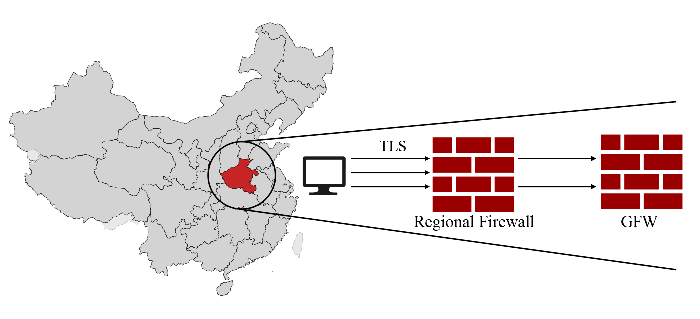
\includegraphics[width=\columnwidth]{figures/two-firewalls.pdf}
  \caption{
    Henan Province has deployed TLS SNI-based and HTTP Host-based censorship middleboxes
    that inspect and block traffic exiting the province.
    % Henan Firewall maintains a blocklist that is ten times larger than the national GFW's.
    }
  \label{fig:two-firewalls}
\end{figure}

%\noindent\textbf{Unraveling Censorship in Henan.} Henan, being the third-largest
%province by population and a pivotal tech hub in China, is home to several
%high-tech industries, including major Apple iPhone manufacturing units. The
%province has been a cradle for firms that developed censorship software for the
%government, such as the infamous Green Dam Youth Escort
%software~\cite{greendam}. Given this background, Henan could be an ideal
%location for piloting new censorship initiatives. Recent social and political
%disturbances~\cite{Security88:online, HowChine24:online} in the region can also
%be attributed to the increased censorship measures in the region. While the
%exact motives for the ramp-up in censorship activities in Henan~\textemdash{}
%whether they serve to mitigate the region's unrest or are part of a larger
%scheme to regionalize censorship across China~\textemdash{} are not entirely
%clear, the identification of a regional firewall in Henan is a noteworthy
%development in the progression of China's censorship framework, hinting more
%towards a rather decentralized and localized censorship approach.

%\noindent\textbf{China's potential shift towards decentralized control.}
%Previous studies on regional censorship in China~\cite{Xu2011a, Wright2012a} are
%limited and outdated. Early research, such as the work by Xu et
%al.~\cite{Xu2011a} almost a decade ago, noted the presence of keyword censorship
%middleboxes in certain provinces but found no major deviations in their behavior
%from national policies. Wright's~\cite{Wright2012a} 2012 paper on varying DNS
%server responses across China was synthesized by a model of DNS censorship that
%adheres to a centralized-control approach by subsequent works~\cite{Hoang2021a,
%Anonymous2020a} in the area. Overall, the literature suggests that censorship
%mechanisms in China generally conform to a central policy. Thus, the recent
%observations of independently operating regional firewalling represent a novel
%and significant departure from the norm, highlighting the need for further
%investigation into this phenomenon.

We conduct a longitudinal study to understand the content blocked by the Henan
Firewall and how it differs from the content blocked by the GFW
(\autoref{sec:blocklists}).  Between November 2023 and March 2025 (with a
measurement gap between March and October 2024), we tested Tranco top
one~million domains on a daily basis, and tested CZDS 227~million domains on a
weekly basis.
% across seven provinces and municipalities in China.
We find that the Henan Firewall employs more aggressive and volatile blocking
policies than the GFW.  The Henan Firewall blocked a cumulative 4.2~million
domains, more than five times the size of the GFW's cumulative blocklist.  A key
reason for this was its blocking of generic second-level domains (e.g.,
\texttt{*.com.au}).  Our testing also revealed periods where it blocked ten
times more domains than the GFW\@.

% The discovery of a regional TLS firewall in Henan~\cite{Henan-user-report}
% may not a one-off incident that
% hints towards China's potential shift towards a more decentralized approach.
% Be cautious to mention any other regional firewalls. For example, we measured but find no evidence of regional firewalls in Quanzhou.
% There have also been other anecdotal reports of stricter controls
% being implemented in different regions.
% For instance, users have also reported a domain and IP `whitelisting' deployment in the Quanzhou
% region~\cite{NationSt55:online, Anyideaw32:online}.
% Given these developments, we argue that there is a strong case for a thorough investigation
% and a re-look into the regional censorship mechanisms within China.

Based on the observed parsing flaws and injection behaviors, we introduce
circumvention techniques to bypass this regional censorship
(\autoref{sec:circumvention}), which have been implemented by various popular
anti-censorship tools.  The regional censorship in Henan marks one of the first
formally documented cases of a provincial firewall operating autonomously in
China.  We hope our study sounds the alarm to the broader censorship research
community to identify, investigate, and combat the emergence of regional
censorship in China and elsewhere.
% Our code and data is available at
% \url{https://gfw.report/publications/sp25/en}.

% and discuss the implications of regional censorship for the anti-censorship community.


%In this work, we show evidence that China has indeed started deploying
%province-level firewalls that work in conjunction with the main national
%border-level firewall, i.e., the GFW. Our China-wide analysis uncovers the
%emergence of additional regional firewalls, with the first detected instance of
%a regional TLS firewall in Henan.



% \amir{you dont talk about OTHER provinces. either you say that you tested others and there was no evidence of regional cens by them, or something. but you cant not mention other provinces}

%In summary, this paper makes the following contributions:
%
%\begin{itemize}
%
%	\item We show evidence that China has deployed province-level firewalls in
%		Henan that work in conjunction with the GFW deployed nation-wide.
%
%	\item We fingerprint and compare the packets injected by the Henan Firewall
%		and the GFW.
%
%	\item We perform a longitudinal experiment to document the evolution of the
%		blocklist of the two firewalls (Henan and GFW) and show that the Henan
%		Firewall is ten times larger and more frequently updated.
%
%	\item
%
%	\item
%\end{itemize}
%

\section{Background and Related Work}

\subsection{The Great Firewall of China (GFW)}
The Great Firewall of China (GFW) is a set of
different censorship mechanisms and devices deployed in China.
The GFW utilizes a network of middleboxes distributed across China's border autonomous systems (ASes)
to inspect and block Internet traffic~\cite{Xu2011a}.
The GFW not only blocks access to specific websites and services,
but also tries to identify and block attempts to bypass its censorship.

\parhead{Website censorship.}
To block access to specific websites and services,
the GFW often employs a combination of techniques,
including DNS injection~\cite{Duan2012a, Hoang2021a},
HTTP Host-based filtering~\cite{Rambert2021a},
TLS SNI/ESNI-based filtering~\cite{Chai2019a, 2022-tls-blocking, Hoang2024a, Bock2020ESNI},
and IP address blocking~\cite[\S4]{Chai2019a}.

To censor DNS traffic,
the GFW operates \textit{on-path} to inject forged DNS responses with wrong IP addresses
to block access to specific domains~\cite{Farnan2016a,Anonymous2014a,Hoang2021a,Anonymous2020a,Fan2025a}.
Early reports from 2002 documented that the GFW used a single wrong IP address in its forged responses~\cite{Dong2002a,Zittrain2003a}.
Over time, this evolved into a more sophisticated system employing an increasing number of fake
addresses and expanding the list of blocked domains~\cite{Lowe2007a, Anonymous2014a, Anonymous2020a, Hoang2021a}.
Researchers have uncovered memory disclosure vulnerabilities in the GFW's injection system~\cite{gfw-looking-glass-post,Sakamoto2024a,Fan2025a}.

To censor HTTP and TLS traffic,
the GFW statefully inspects unencrypted text in the connection.
Upon detecting a censored domain in
a HTTP request's Host field or in a TLS ClientHello's Server Name Indication (SNI) extension,
the GFW injects TCP \texttt{RST}
packets to both sides of the connection to tear it down~\cite{tang2016depth,Wang2017a,Bock2021b,Hoang2024a,Clayton2006a}.
\autoref{fig:waterfall-diag} shows the GFW's operation on a connection
containing a forbidden domain name in the SNI of the TLS Client Hello.

The GFW often operates bidirectionally,
meaning both traffic coming into the country and leaving the country
can trigger its censorship~\cite{Sparks2012a,Anonymous2020a,Hoang2024a}.
The bidirectional operation of censorship middleboxes
has enabled researchers to
measure censorship from outside the country~\cite{Marczak2015a, Pearce2017b, Hoang2021a}.


Projects such as OONI~\cite{Filasto2012a},
Censored Planet~\cite{Raman2020c},
and ICLab~\cite{Niaki2020a} have been measuring censorship globally for years.
To monitor website censorship in China,
several large-scale projects have been developed,
including the GreatFire Analyzer~\cite{greatfire_analyzer},
Blocky~\cite{greatfire_blocky},
GFWatch~\cite{Hoang2021a},
and GFWeb~\cite{Hoang2024a}.
While longitudinal and large scale studies are excellent at tracking and understanding
the blocklist changes in the GFW,
sometimes a revisit of the existing censorship mechanisms could still reveal new updates by the censor.
For example,
Bock et~al.~\cite{Bock2021c} discovered secondary TLS censorship middleboxes in China
that had operated undetected until an in-depth analysis revealed them.


\parhead{Proxy censorship.}
Blocking access to websites is not enough to prevent users from accessing
censored content,
as users can use circumvention tools to bypass censorship.
There has thus been a seemingly endless cat-and-mouse game between the GFW and the Internet users in China~\cite{cat-and-mouse}.
For example,
the GFW employs active probing techniques to identify
and block circumvention tools,
such at Tor~\cite{Winter-obfs2-probe,Winter2012a,knock-knock-tor,Ensafi2015b,Dunna2018a}
and Shadowsocks~\cite{Alice2020a}~\cite[\S 5]{Wu2023a},
which have been successfully defended against~\cite{Anonymous2021ShadowsocksAdvise,Anonymous2021ShadowsocksTutorial,Frolov2020a,Frolov2020b}.
The GFW also conducts traffic analysis to identify and block fully encrypted proxies~\cite{Wu2023a}.


\parhead{Other censorship mechanisms.}
There have also been unique components of China's censorship that appear
separate from the GFW's censorship against websites and proxies.
Notably,
in 2015, researchers discovered the ``Great Cannon'' of China,
which injected Javascript into HTTP traffic in order to
co-opt victim browsers into participating in a denial-of-service attack against
specific hosts~\cite{Marczak2015a}.

\subsection{Regional Variation in Censorship}

Localized or decentralized censorship mechanisms are common in countries with
strict censorship policies. In Russia, thousands of privately owned ISPs each
implement their own filtering mechanisms, resulting in a varied censorship
landscape~\cite{Xue2022b,Ortwein2023a,Ramesh2020a}.
Similarly, in India, researchers have shown that ISPs differ significantly in their implementation of government censorship orders,
leading to fragmented censorship across the country~\cite{Yadav2018a}.

However,
prior work has suggested that
China's censorship systems and policies are largely uniform and centralized across the country.
%
In 2011, Xu et al.~\cite{Xu2011a} measured the location of censorship devices in China.
They found that China's keyword-censoring middleboxes were largely at the edges of the network
and employed rules in line with nationwide blocking policies of that time.
In 2012, Wright~\cite{Wright2012a} performed a small-scale study on DNS
censorship in China, finding that DNS responses to queries varied across the country.
However, this work did not account for other possible causes of the variation in DNS responses
(e.g. geolocation-based load balancing, or changes in DNS configuration).
In 2018,
Bao et al.~\cite{Bao2018a} measured DNS injection variances in China from residential and cellular IP addresses.
Internet-wide and longitudinal measurements
have revealed China's
uniform and coordinated management of
censorship policies~\cite{Anonymous2020a, Hoang2021a, Wu2023a, Hoang2024a},
software updates~\cite[\S4.5]{Sakamoto2024a}~\cite[\S VII]{Fan2025a},
and infrastructures~\cite[\S3.4]{Alice2020a}~\cite[\S 5]{Anonymous2020a}.

\begin{table*}[t]
  \small
  \centering
  \caption{Experiment timeline and vantage points.
  In total,
  we used
  14 VPSes in China VPS Cloud (CVC, AS4837) in Zhengzhou, Henan Province (HN),
  six VPSes in Akamai Linode (LD, AS63949) in San Francisco (SF), Singapore (SG) and Seattle (SE),
  12 VPSes in Tencent Cloud (TC, AS45090) in
  Beijing (BJ),
  Shanghai (SH),
  Chongqing (CQ),
  Guangzhou, Guangdong Province (GZ),
  Chengdu, Sichuan Province (CD),
  Nanjing, Jiangsu Province (NJ),
  and one bare metal network tap server (TAP) in a U.S. university.
  }
  \begin{tabular}{llr@{~}llll}
    \toprule
    Experiments & Time Span & \multicolumn{2}{l}{Duration}        & China Vantage Points & External Vantage Points & Sections                  \\
    \midrule
    Identification & 7/10/24 & 1 & day & 12 (TC), 2 (CVC: HN) & 4 (LD: SG,SE)  & \S\ref{sec:detection} \\
    Characterization & 10/2/23 -- 11/12/24 & 13 & months & 2 (CVC: HN) & 1 (LD: SF), 3 (TC: GZ,BJ,SH)  & \S\ref{sec:characterization} \\
    Traffic Analysis & 10/31/24 & 1 & hour & - & 1 (TAP: US)& \S\ref{sec:parsing-logic}   \\
    Locating & 10/2/23 -- 12/8/23 & 2 & months & 1 (CVC: HN), 1 (TC: GZ) & 1 (LD: SF) & \S\ref{sec:location}   \\
    Blocklist & \makecell{11/5/23 -- 3/5/24 \& \\ 10/07/24 -- 3/31/25} & 9 & months & 14 (CVC: HN), 2 (TC: GZ) & 2 (LD: SF)& \S\ref{sec:blocklists}   \\
    \bottomrule
  \end{tabular}
  \label{table:exp-summary}
\end{table*}

\section{Detecting Regional Censorship}
\label{sec:detection}

\begin{figure}[t!]
  \centering
  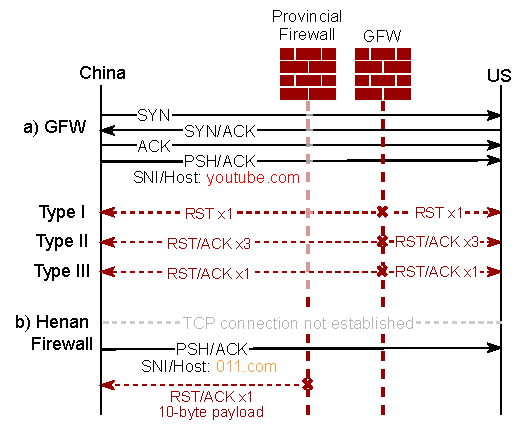
\includegraphics[width=\columnwidth]{figures/waterfall-diag.pdf}
  \caption{
    Overview of the Henan Firewall and the three different types of GFW.
    One can trigger and study each censorship mechanism individually
    by putting exclusively censored domains in the SNI or HTTP Host field of a probe.
    For example,
    as of April~2024,
    \texttt{011.com} was exclusively blocked by the Henan Firewall,
    and \texttt{youtube.com} was exclusively blocked by the GFW.
  }
  \label{fig:waterfall-diag}
\end{figure}

Anti-censorship researchers outside of China often rely on local user reports
to learn about the new censorship shifts and upgrades in China.
This is partially because of the difficulty for researchers to
obtain a diverse range of vantage points inside China
and then constantly monitor various Internet services and protocols.
Encouragingly,
online discussion forums---such as
Net4People BBS~\cite{net4people_bbs_issues},
NTC Party forum~\cite{ntc_party_forum}, and
the GitHub issue pages of popular anti-censorship tools
such as Xray~\cite{xtls_xray_core_issues}, V2Ray~\cite{v2fly_v2ray_core_issues}, sing-box~\cite{sagernet_sing_box_issues},
and Hysteria~\cite{apernet_hysteria_issues}---enable users to report new censorship
behaviors as soon as they encounter
them and allow researchers to investigate those reports promptly~\cite{cat-and-mouse}.

This crowdsourced, collaborative approach has also been effective in identifying and combating the provincial censorship in Henan.
In particular,
our study started with reports from a group of users in Henan who were
unable to access certain websites~\cite{Henan-user-report, net4people442, net4people416, ghostcomment, tsinbei_tcp_timestamps}.
We then obtained a server in the Henan Province
and confirmed the presence of a regional firewall.
In particular,
as illustrated in~\autoref{fig:waterfall-diag},
we found that the regional Henan Firewall
blocked TLS and HTTP connections for some Server Name Indication (SNI) and HTTP Host values,
but it operated differently than the GFW.
Most distinctively,
the regional firewall in Henan blocks a TCP connection by injecting one TCP \texttt{RST+ACK} packet
containing a fixed 10-byte payload to the client.
The unique payload of TCP \texttt{RST} packet differentiates the Henan Firewall
from all three types of packets injected by the GFW.

The discovery of regional censorship in Henan province led to a natural question:
have other provinces in China deployed the same or similar regional censorship?
Below, we explore this question with measurement across the country.


\subsection{Experiment}

Our goal is to quantify the regional variation of TLS censorship across China
by comparing the number of domains blocked between each pair of hosts inside or outside of China.
%
As summarized by the second row of~\autoref{table:exp-summary},
we obtained two vantage points in each of the seven cities in China,
including Shanghai, Beijing, Chongqing,
Guangzhou (Guangdong Province),
Nanjing (Jiangsu Province),
Chengdu (Sichuan Province),
and Zhengzhou (in Henan Province).
We also setup two VPSes in each of the three locations outside of China:
Seattle (U.S.),
San Francisco (U.S.),
and Singapore.
Our selection of vantage points was
guided by a set of ethical considerations detailed in~\autoref{sec:ethics}.

For the two VPSes in each location inside or outside of China,
we used one as a client and the other as a \emph{sink server}.
The sink servers were configured to
accept TCP handshakes on all ports between 1 and 65535.
They would acknowledge the TCP data sent to them,
but would never send any TCP payload back to the client.
We configured \texttt{iptables} rules on both the client and sink servers to drop any outgoing \texttt{RST} packets.
This way,
any \texttt{RST} packets received on either end must be injected by some middleboxes on the network path.
We could thus confirm the presence of censorship by checking whether the TCP connection was being reset.

We then sent TLS traffic with various SNI values between each pair of the clients and sink servers
on July~10, 2024.
In particular,
we used the top 10,000 domains
from the Tranco list~\cite{LePochat2019tranco} 5YZ7N for testing.\footnote{Tranco list ID 5YZ7N, obtained on August~15, 2023: \url{https://tranco-list.eu/list/5YZ7N/1000000}.}
To reduce the chances of false negatives due to packet loss,
we repeated our test three times on the same day and let the OS to control retransmissions of the packets.

\parhead{Limitations.}
Ideally,
we would liked to use a diverse set of vantage points to identify potential regional censorship in China.
However,
due to the difficulty of obtaining VPSes in China,
we have only been able to obtain vantage points in a limited number of locations and ASes.
While using residential vantage points would have allowed us to observe potential middleboxes
from more network locations in China,
this could put potential risks on uninformed users and providers of residential proxies~\cite{Mi2019-resident-evil}.
For this reason,
we focus on using two large VPS providers in China,
China VPS Cloud and Tencent Cloud,
to avoid risks or persecution to individuals.
We utilized all available locations these two VPS providers offered to maximize our coverage.
We acknowledge that our results are limited to measuring TLS censorship,
which could potentially miss regional censorship of other protocols.
Additionally, due to a configuration error,
we did not test using our client in Singapore,
potentially missing bidirectional censorship from that perspective.

\begin{figure}[t]
  \centering
  \includegraphics[]{figures/client-to-sink-server-data-matrix.pdf}
  \caption{
    The matrix shows the number of domains blocked between each pair of hosts in various locations.
%
    For each host pair,
    we sent TLS ClientHello messages with SNI values
    of the top 10,000 domains from the Tranco list~\cite{LePochat2019tranco} 5YZ7N,
    generated on August~15, 2023.
%
    The result suggests that
    1) regional censorship in Henan province exists
    evidenced by the non-zero number of blocked domains when testing from Zhengzhou, Henan to
    sink servers in other regions of China;
    2) the censorship in Henan is not bidirectional,
    as initiating TLS connections from the outside to Henan did not trigger any blocking;
    3) the GFW maintains a blocklist that is only censored when accessed from within China,
    as evidenced by the differences in the numbers of blocked domains when testing inside-out and outside-in.
  }
  \label{fig:indentification-exp}
\end{figure}


\begin{figure*}[t]
  \centering
  % -------- Henan ----------
  \begin{subfigure}[b]{0.48\textwidth}
    \centering
    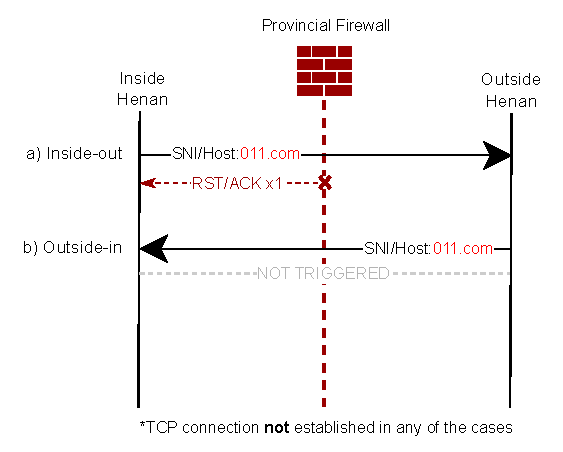
\includegraphics[width=\linewidth]{figures/henan-inside-outside.pdf}
    \caption{Henan Firewall}
    \label{fig:henan-inside-outside}
  \end{subfigure}
  \hfill
  % -------- GFW -----------
  \begin{subfigure}[b]{0.48\textwidth}
    \centering
    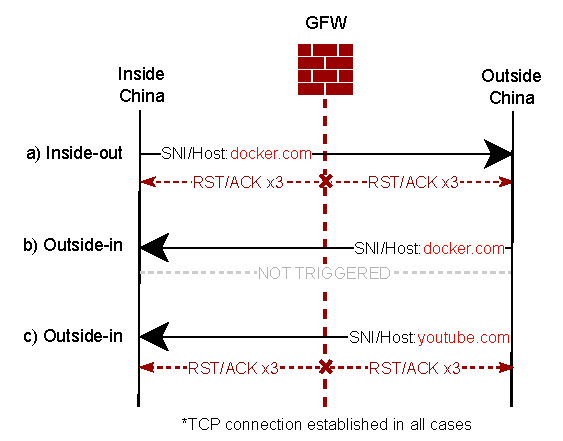
\includegraphics[width=\linewidth]{figures/gfw-inside-outside.pdf}
    \caption{GFW}
    \label{fig:gfw-inside-outside}
  \end{subfigure}

  \caption{
    (a) The Henan Firewall does not censor inbound TLS or HTTP traffic to Henan,
      contracting the bidirectional censorship employed by the GFW.
    (b) The GFW's TLS and HTTP censorship machines inspect bidirectional traffic
    coming in and out of China; however, certain domains are only censored when accessed from within China.
    In this example, while a TLS ClientHello with SNI value \texttt{docker.com}
    can trigger the three TCP \texttt{RST} packets by the GFW when sent from within China,
    it does not trigger any blocking when sent from outside of China.
  }

  \label{fig:inside-outside-comparison}
\end{figure*}

\subsection{Results}


\autoref{fig:indentification-exp} shows the number of
blocked domains between different locations.
We first observe that,
connections originating from China to our sink servers in Singapore and the U.S. %Seattle
were almost equally impacted by the national-level Great Firewall of China (GFW),
with around 479 out of the 10,000 domains blocked.
The most significant blocking was observed in Zhengzhou,
the capital of Henan province, where both provincial (Henan) and national (GFW)
censorship mechanisms contributed to the high figure.

% Readme in comfirmation folder has the command to generate this percentage
Traffic leaving Henan is affected by the regional firewall,
regardless of the sink server location, even to other regions within China.
On average, 122 domains were blocked by the Henan Firewall.
We did not observe any blocking of TLS connections within Henan itself;
however, since both of our client and sink servers were in the same data center,
we can only cautiously conclude that the Henan Firewall does not
affect internal traffic within this data center.

When connections were made from Zhengzhou, Henan Province,
to locations outside China (Singapore and Seattle),
a total of 594 domains were blocked.
This indicates the simultaneous operation of two
firewalls with independent blocklists, with the Henan Firewall
intercepting traffic before it reaches the GFW and thus,
increasing the total number of domains that are blocked.
We, however, did not observe any blocking of connections
from other client locations in China to Henan or other
sink server regions within China. This finding suggests
that the \emph{Henan Firewall is the first known
deployment of a regional firewall in China.}

Moreover, as presented in the last row
of~\autoref{fig:indentification-exp},
tests from the U.S. to various locations in China
consistently identified the same 411 domains blocked by the GFW,
with only one exception:
tests from the U.S. to Jiangsu Province detected 440 blocked domains.
Further analysis indicates that the additional 29 domains blocked in the outside-in direction
for Jiangsu is a subset of the 479 domains blocked by the GFW in the inside-out direction.
This finding suggests that the additional censorship of these 29 domains
likely does not reflect regional censorship specific to Jiangsu.
Instead, it indicates that the GFW is configured to block these domains bidirectionally within Jiangsu.

Overall, these results are particularly noteworthy as they show the
infeasibility of remote measurements to trigger the regional firewalls and
more importantly, the asymmetric behavior of the GFW.
In particular, while 479 domains were blocked on average when
connections were initiated from within China, only 411 domains
were blocked when connections were initiated from outside China.
This discrepancy suggests that the GFW enforces a different blocklist
for traffic originating from within China. Until recently,
it was widely believed that the GFW operated symmetrically,
triggering and applying the same blocklist to traffic regardless of direction.
However, recent work has suggested this assumption is incorrect~\cite{Hoang2024a},
and our findings here are consistent with this recent result.


We note that both the GFW and the Henan Firewall exhibit asymmetric interference to varying degrees. As shown in~\autoref{fig:henan-inside-outside}, while traffic going out of Henan is subject to the regional firewall (inside-out),
inbound traffic (outside-in) to Henan does not trigger the regional firewall at all. This stands in contrast to the GFW, which, although bidirectional, behaves asymmetrically based on the domains queried.

\autoref{fig:gfw-inside-outside} provides a clear example of this behavior. When a TLS ClientHello with SNI value \texttt{docker.com}, in our case, is sent from within China (inside-out), the GFW triggers blocking via three TCP \texttt{RST} packets. However, when the same TLS ClientHello is sent from outside of China (outside-in), the GFW does not trigger any blocking. On the other hand, when a TLS ClientHello packet with the SNI value \texttt{youtube.com}, in this example, is sent, the GFW triggers blocking in both scenarios: whether the packet is sent from inside or outside China. This behavior demonstrates an apparent blocklist of domains that are exclusively censored by the GFW when accessed from within China.

In our experiment designed to detect any regional censorship, we inadvertently uncovered a significant aspect of the GFW's operational mechanics that has only recently been documented~\cite{Hoang2024a}. The newly observed asymmetric nature of the GFW and regional firewalls highlights the critical need for inside-out measurements to fully capture the extent and nuances of censorship. Relying solely on remote measurements, as is common in many other studies, fails to provide a comprehensive picture of such censorship events.

To further substantiate the asymmetric behavior of the GFW, we provide a list of domains that are exclusively blocked when sending TLS ClientHello messages from within China, as shown in ~\autoref{table:only-censored-inside-out}. In our experiment, 68 out of the 10,000 domains did not trigger any censorship when tested from outside China but only were blocked when probed from inside China. These domains include popular websites such as \texttt{google.com}, \texttt{nyt.com}, and \texttt{docker.com}. The list serves as concrete evidence of the selective enforcement of the GFW's blocklist based on the origin of the traffic and the domain in question.




\begin{table}[t]
  \centering
  \small
  \caption{
    A sample of domains that are exclusively blocked by the GFW when sending TLS ClientHello messages from within China.
    These domains did not trigger censorship when sent from outside China to within,
    as of July 10, 2024.
  %   wc -l ../confirmation/only-censored-*
  %  68 ../confirmation/only-censored-inside-out.txt
  %   0 ../confirmation/only-censored-outside-in.txt
  Among the 10,000 Tranco top domains we tested, 68 domains were exclusively blocked inside-out
  and no domains were exclusively blocked outside-in.
  }
  \begin{tabular}{l|l|l}
    \toprule
    binance.com      & godaddy.com   & note.com       \\
    cdninstagram.com & google.com    & nyt.com        \\
    docker.com       & google.com.hk & tiktokcdn.com  \\
    gmail.com        & linktr.ee     & torproject.org \\
    \bottomrule
\end{tabular}
  \label{table:only-censored-inside-out}
\end{table}


\section{Characterizing the Censorship Devices}
\label{sec:characterization}

Since October~2023,
we conducted a series of experiments to characterize censorship devices
and understand the differences between the Great Firewall (GFW)
and Henan regional censorship devices.
In this section, we answer several research questions:
where are the regional censorship devices located?
What packets can trigger the Henan SNI Firewall?
Which ports are monitored by the Henan Firewall?
Does the TCP \texttt{RST} injections have any specific fingerprints?
And does the Henan Firewall induce residual censorship?

\subsection{Methodology}
\label{sec:methodology}

We developed a methodology tailored to the specific characteristics of two firewalls, i.e., regional and national, as discussed earlier. To precisely assess the impact of each firewall, our approach involves isolating and analyzing these two systems individually. This method, which was devised based on our preliminary observations, serves as the foundation for our comprehensive measurement experiments. Key aspects of our methodology are outlined below.

\parhead{Obtaining Vantage Points.}
In total we use 10 vantage points in Zhengzhou, China (in Henan) acquired via China VPS Cloud (AS 4837),
two VPSes in Guangzhou, one in Beijing, and one in Shanghai via Tencent Cloud (AS 45090),
and two VPSes in San Francisco, U.S. through Akamai's Linode (AS 63949).
The VPSes in Guangzhou, Beijing, Shanghai and San Francisco served as sink servers that were programmed
to listen on ports 1 to 65535 and accept TCP connections but did not send any other data back to the sender.
All our machines ran Ubuntu 22.04, and we verified their advertised locations using the IP2Location~\cite{ip2location} database.
We have summarized the timeline of our experiments and the vantage points used in each in~\autoref{table:exp-summary}.

\parhead{Dropping Outgoing RSTs on the VPSes.}
We configured \texttt{iptables} rules on both the client and sink servers to drop all outgoing \texttt{RST} packets.
This configuration ensures that any \texttt{RST} packet received by the client side can be reliably attributed to middlebox injections.

\parhead{Triggering TLS SNI-based Censorship.}
We trigger censorship by sending a TLS ClientHello with potentially censored domain names in the SNI field.
Since the sink servers are configured to not respond with any data packets
and not tear down connections before observing a \texttt{FIN} or a \texttt{RST} packet,
we expect any \texttt{RST} packets received are indeed injected packets from a firewall.
We mark a domain name as censored if a \texttt{RST} packet is received for a TLS ClientHello containing the domain name.

\parhead{Triggering HTTP Host-based Censorship.}
To trigger HTTP censorship,
we sent HTTP GET requests with the forbidden domain name in the Host header of the request:
% request := fmt.Sprintf("GET / HTTP/1.1\r\nHost: %s\r\n", host)
\begin{verbatim}
  GET / HTTP/1.1\r\nHost: example.com\r\n
\end{verbatim}
% We note the minimal HTTP request trigger the Henan Firewall is:
% \begin{verbatim}
%   GET / HTTP/1.1\r\nHost: example.com\r
% \end{verbatim}
% or
% \begin{verbatim}
%   GET / HTTP/1.1\r\nHost: example.com\n
% \end{verbatim}
While later we found that the Henan Firewall does not require a full TCP handshake to trigger blocking,
we still complete a TCP handshake before sending the HTTP request,
making our testing methods consistent against the Henan Firewall and the GFW.
We mark a domain name as censored if a \texttt{RST} packet is received for an HTTP GET request containing the domain name.


\parhead{Isolating the Henan Firewall.}
To distinguish Henan Firewall responses from the GFW's, we identify several
fingerprints unique to each firewall.
Prior work has documented the GFW disrupts
connections by injecting up to three \texttt{RST+ACK} to both sides of the connection
whenever a TLS ClientHello message with a forbidden Server Name Indication field is observed~\cite{Chai2019a,Bock2020b}.
In contrast, the Henan Firewall injects a single \texttt{RST+ACK} packet
to only the client side of a connection.
In addition, the Henan Firewall's \texttt{RST+ACK} packet contains a payload,
making it easy to distinguish from GFW responses.
We expand on this in~\autoref{sec:how-block}.

Finally, we send probes from vantage points in Henan to servers in Guangzhou, Beijing, and Shanghai to make sure that our traffic is not routed outside China (where it may encounter the GFW) but is still subject to the regional firewall in Henan.

\parhead{Limitations.}
Our measurements in Henan Province are limited to a single Autonomous System (AS),
China Unicom (AS~4837),
due to the difficulty of obtaining diverse vantage points in China
that could be ethically used for censorship measurement.
Consequently,
our empirical findings are confined to this single Internet Service Provider (ISP),
limiting our ability to confirm or characterize censorship practices across other ISPs or ASes in Henan.

While user reports suggest that
ISPs in Henan employ region-specific censorship,
the censorship implementations are reportedly distinct~\cite{Henan-user-report-1}.
For instance, Github user 5e2t reported that China Mobile Henan censored
traffic on its cellular network and was capable of reassembling closely spaced TCP packets~\cite{Henan-user-report-1},
which differs from the behavior we observed on China Unicom in~\autoref{sec:parsing-logic}.
Therefore, our results should be interpreted as reflective only of China Unicom Henan's censorship implementation,
not necessarily indicative of province-wide practices across all~ISPs.

\subsection{What Traffic Is Targeted}
\label{sec:what-targeted}

\parhead{Does the Henan Firewall sample traffic to monitor and censor?}
The censor has been observed to only monitor and censor a fraction of traffic,
potentially as a way to reduce the computation load on its censorship devices~\cite[\S 6.3]{Wu2023a}.
We, however, did not observe any traffic sampling
or probabilistic blocking behaviors from the Henan Firewall.
We observed that the Henan Firewall consistently blocked domains listed on its blocklist.
We sent 1,000 consecutive ClientHello messages containing a
forbidden domain name, each request made over a unique port pair with small delays.
We received the TCP \texttt{RST} packets for every connection we made,
indicating a 100\% triggering rate of censorship for censored domains of the Henan Firewall.

\parhead{What ports does the Henan Firewall monitor?}
Previous works have shown that the GFW TLS ESNI censorship middleboxes monitor all ports i.e. 1-65535~\cite{Bock2020ESNI}.
To measure the Henan Firewall,
we sent TLS ClientHello messages,
with a known blocked SNI to all ports of our sink server in Guangzhou, China.
We found that the Henan Firewall, similar to the GFW, monitors TLS traffic going to any TCP port number, ranging between 1 and 65535.

\parhead{Is the Henan Firewall bidirectional?}
Owing to the inherent limitations of obtaining vantage points in a censored region,
researchers typically opt for performing measurements from the outside in rather than inside out.
Particularly in China,
works that study the GFW~\cite{Hoang2021a,Anonymous2020a,Hoang2024a} used vantage points
outside China because of its bidirectional nature.
%
However,
as mentioned in~\autoref{sec:detection},
sending probes from outside China does not trigger the Henan Firewall
as it only censors traffic going out of Henan.
As shown in~\autoref{fig:indentification-exp},
we tested this by sending TLS ClientHello messages
with different SNI values in the Tranco list~\cite{LePochat2019tranco} 5YZ7N,
between nodes in Henan and nodes in other regions of China.
We found that only traffic going out of Henan was blocked by the regional firewall.
Similar asymmetric blocking behaviors were also observed in the GFW
by prior work~\cite{Hoang2024a, Bock2020ESNI}.

\subsection{How the Henan Firewall Parses Connections}
\label{sec:parsing-logic}

In this section,
we look at the parsing logic of the Henan Firewall and the GFW.
We perform experiments to check the TCP handshake requirements for triggering the Henan Firewall and the GFW.
We also use DPYProxy~\cite{Niere2023a} to test for TCP and TLS reassembly capabilities,
as well as the presence of residual censorship in the two firewalls.
We summarize our findings in~\autoref{table:parsing-logic}.


\begin{table}[t]
  \caption{Parsing logic of the GFW and the Henan Firewall.
  The Henan Firewall appears to be stateless
  and less robust against typical network variability than the GFW.
  }
  \label{table:parsing-logic}
  \small
  \centering
  \begin{tabular}{lcc}
    \toprule
    & \textbf{GFW} & \textbf{Henan Firewall} \\
    \midrule
    Require SYN & \cmark & \xmark \\
    Require SYN+ACK  & \xmark & \xmark \\
    TCP Reassembly & \cmark & \xmark \\
    TLS Reassembly & \xmark & \xmark\\
    TCP Header Length & Arbitrary & 20~bytes Only\\
    \bottomrule
  \end{tabular}
\end{table}


\parhead{TCP handshake completeness requirements.}
The middleboxes designers often need to make a trade-off
between the complexity of the parsing logic
and the efficiency of the traffic analysis operations.
For example,
due to asymmetric routing nature of the Internet,
and the fact that Henan Firewall and the GFW are not always immediate neighbors of the client or the server (as shown in~\autoref{table:centrace-results}),
the middleboxes may only be able to observe flows in one direction.
This nature often makes the middleboxes' designers not require to observe a complete TCP three-way handshake
to track TCP connection and conduct censorship.
On October~10, 2024,
we tested the requirements of the TCP handshake completeness for the Henan Firewall and the GFW from our vantage point in Henan.
We sent a single TCP packet whose payload is a TLS Clienthello message contained a forbidden domain name \texttt{011.com} as the SNI,
preceded by 1) a SYN packet from client, or 2) a SYN packet from the client and a SYN+ACK packet from the server, or 3) no packet at all.

As summarized in~\autoref{table:parsing-logic},
while the GFW requires to observe a SYN packet from the client (but not a SYN+ACK packet from the server)
to trigger the censorship~\cite{Hoang2024a},
the Henan Firewall does not require to observe any TCP handshake packet to be triggered.

\parhead{TCP segmentation.}
TCP segmentation enables the splitting of larger TCP payloads into smaller ones.
In the context of circumvention, splitting a TLS ClientHello message into multiple TCP segments
has been used to confuse stateless censors that do not reassemble packets.
However, we confirm that the GFW performs TCP reassembly and thus, is stateful.
On the other hand, we found that the Henan Firewall does not perform TCP reassembly and thus,
it is possible to bypass it by splitting the TCP payload of the ClientHello into multiple TCP segments,
with the SNI distributed between the segments.
We tested this by initiating a TLS connection from our vantage point in Henan to our VPS in Guangzhou
with a forbidden SNI and splitting the ClientHello into two segments,
with the second segment containing the forbidden domain name.
We observed that while a complete ClientHello message was blocked by the Henan Firewall,
not putting a complete SNI extension in the first segment would bypass the Henan Firewall.


\parhead{TLS fragmentation.}
While TCP segmentation has been long known to be used to bypass stateless censors,
the use of TLS fragmentation was only recently analyzed by Niere et al.~\cite{Niere2023a}
and implemented in their DPYProxy tool.
Before a TLS message is encapsulated within a TCP segment,
it is first enclosed in what is known as a TLS record.
Given that the maximum size of a TLS message exceeds the maximum allowable size for a TLS record,
the TLS standard permits the division of TLS messages across several TLS records.
Niere et al.~\cite{Niere2023a} found that the GFW did not perform TLS reassembly
and it is thus possible to bypass it by fragmenting TLS ClientHello messages over multiple TLS records,
wherein the SNI is split into multiple TLS segments within the same TCP payload.
We confirm that,
as of April 4, 2024,
both the Henan Firewall and the GFW do not perform TLS reassembly and thus,
it is possible to bypass them via TLS ClientHello fragmentation.

% python3 plot.py header_len.jsonl --out "header-length.pdf" --no-show
% Total TCP packets: 23,074,696,071
% Total TLS packets: 4,993,645,322
% Percentage of TCP packets with header length 20: 22.28%
% Percentage of TLS packets with header length 20: 19.46%


\begin{figure}[t!]
  \centering
  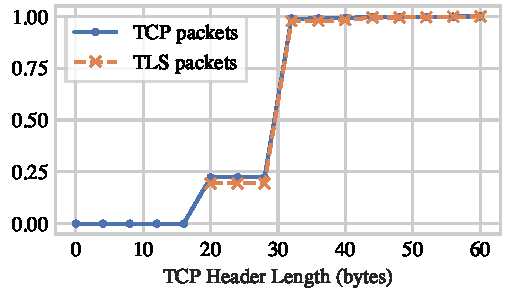
\includegraphics[]{figures/header-length.pdf}
  \caption{
  The distribution of the TCP header length fields of all TCP and TLS packets
  during a one-hour captured on a university network on October 31, 2024.
  In total,
  we captured approximately 23.1~billion TCP packets and 5.0~billion TLS packets.
  Only 22\% of any TCP packets have a header length of 20 bytes,
  while only 19\% of any TLS packets have a header length of 20 bytes.
  This evaluation result suggests that the Henan Firewall has only being able to
  censor around 20\% of the targeted connections.
  }
  \label{fig:header-length}
\end{figure}


\parhead{TCP header length has to be 20~bytes.}
The four most significant bits of the 13th byte of the TCP header represent the TCP Data Offset,
which specifies the length of the TCP header in 32-bit words.
The minimum value of the TCP Data Offset field is $5$ words (20~bytes)
when no TCP options are present,
and the maximum value is $15$ words (60~bytes).

We found that the Henan Firewall required the TCP header length
to be exactly 20~bytes to correctly parse and block the TLS ClientHello or HTTP request messages.
%
% util/tcp-options
We tested this by sending forbidden messages
(e.g. TLS ClientHello messages with a forbidden SNI \texttt{011.com})
from our vantage point in Henan to our sink server in Guangzhou
on October 17, 2024,
with different TCP options set in their TCP headers.
While varying the TCP header length,
we made sure that the TCP options are always a multiple of four~bytes
to comply with the 32-bit word alignment requirement of TCP header.
The TCP options we tested include common TCP ones like
Maximum Segment Size (MSS), Window Scale, Timestamps,
Selective Acknowledgment Permitted (SAckOk),
No Option (NOP), End of Option List (EOL),
as well as self-defined TCP options that are not commonly used.
We found that as long as any TCP option was set,
the Henan Firewall did not block the connection.

% header-length
An intuitive hypothesis to explain this strange behavior is that
the Henan Firewall does not parse the TCP header length field in the TCP header,
and falsely assumes that the TCP header length is always 20~bytes.
This way,
when a TCP header has more than 20~bytes due to TCP options,
it will treat the TCP options as part of the TCP payload
and will thus fail to recognize a complete TLS ClientHello or an HTTP request message.
However, we falsified this hypothesis and confirmed the Henan Firewall did parse the TCP header length field.
In particular,
we sent TLS ClientHello messages with a forbidden SNI \texttt{011.com} with no TCP option set in its TCP header,
confirming that this message was blocked by the Henan Firewall.
If the Henan Firewall does not parse the TCP header length field in the TCP header,
then regardless of the TCP header length value we put in the TCP header,
this message should be blocked.
We changed the 4-bit TCP header length field in the TCP header to be all $2^4$ possible values from 0 to 15,
and recomputed the correct TCP checksum for each TCP packet,
and found that the Henan Firewall only blocked a connection when its TCP header length value was $5$ words (20~bytes).
This experiment indicates that \emph{the Henan Firewall did parse the TCP header length field in the TCP header,
but had a condition to only block a connection when its TCP header length is 20~bytes.}

Although we were unable to determine
the rationale behind this condition---possibly an oversight by the censor---it raises an important question about how
much real-world traffic evaded detection due to this condition.
We conducted a test on a university network in the United States.
Specifically,
we used Retina~\cite{wan2022retina} to capture
the TCP header length fields for all traffic on the campus network
over a one-hour period
from 3:56:14~PM to 4:56:14~PM (UTC–7) on October 31, 2024.
In total, we collected 23.1~billion TCP
packets and 5.0~billion TLS packets.
As shown in~\autoref{fig:header-length},
only 22\% of the TCP packets had a header length of 20~bytes, and only 19\% of
the TLS packets had a header length of 20~bytes.
This result suggests that
the Henan Firewall may only be able to censor around 20\% of the targeted connections.
% TODO: explain what OSes do not send TCP options?  There are at least 86 OS
% doesn't have any TCP options, according to the nmap database, however, none of
% them seems to be popular: https://svn.nmap.org/nmap/nmap-os-db

% Ctrl+F for this string: "OPS(O1=%O2=%O3=%O4=%O5=%O6=)"

\subsection{How the Henan Firewall Blocks Traffic}
\label{sec:how-block}

\parhead{Does the Henan Firewall employ residual censorship?}
Residual censorship is a mechanism used by censors in which after a censorship event is detected between two hosts,
the censor continues to block all subsequent connections between the two hosts (SrcIP, DstIP, DstPort - three tuple)
for a certain duration typically 90~s or 180~s.
The phenomenon has been documented by multiple previous works,
studying the GFW~\cite{Bock2021a, Clayton2006a, Rambert2021a}.
We found that the Henan Firewall does not perform any residual censorship.
We were able to make connections with the same three-tuple subsequent to any reset injections from the Henan Firewall.


\parhead{Fingerprinting the injection behaviors.}
Continuing the efforts of fingerprinting the GFW's evolving injection behaviors~\cite{klzgrad2009gfw}~\cite{gfwrev2010http}~\cite[\S 3.1]{Niere2023a}~\cite[\S 7.1.6]{Weaver2009a}~\cite[\S 2.1]{Wang2017a},
we fingerprint the TCP \texttt{RST} packets injected by the GFW and the Henan Firewall.
Using the \texttt{RST} packets collected in~\autoref{sec:location},
we analyze their packet features such as IP~ID, IP~TTL, TCP Flags, TCP Payload, and Payload Length.

\begin{table}[t]
  \caption{
    A comparison of the injection behaviors and packet fingerprints of
    the Henan Firewall and the three types of GFW TCP \texttt{RST} injectors.
    All injections were triggered by TLS SNI-based censorship.
    The IP TTLs shown are the observed values;
    their initial values should be higher.
    The `C' and `S' refer to the client and server.
  }
  % \small
  \centering
  \scriptsize
  \setlength{\tabcolsep}{1pt} % Decrease the horizontal padding between columns

  \begin{tabular}{lcccc}
    \toprule

    % run fingerprint.py *.pcap to get this
    % Unique Fingerprints for All Server->Client reset Packets
    % (Format: (IP.df, TCP.rst, TCP.ack))
    % Fingerprint (0, 1, 0): Count = 77892, TTL Range = 55 - 118, IPID Range = 0 - 0
    % Fingerprint (1, 1, 1): Count = 309333, TTL Range = 39 - 238, IPID Range = 163 - 65119
    % Fingerprint (0, 1, 1): Count = 4366, TTL Range = 248 - 248, IPID Range = 39190 - 39219

    %  \texttt{RST} only DF(0)            \texttt{RST+ACK} DF(1)           \texttt{RST+ACK} DF(0)
    & \textbf{GFW (I)} & \textbf{GFW (II)} &  \textbf{GFW (III)} & \textbf{Henan Firewall} \\
    \midrule
    Observed IP TTL &  55--118 & 39--238 & 248 & 58\\
    IP ID & \begin{bytebox}\x{00}\x{00}\end{bytebox} & \begin{bytebox}\x{00}\x{A3}\end{bytebox} -- \begin{bytebox}\x{FE}\x{5F}\end{bytebox} & \begin{bytebox}\x{99}\x{16}\end{bytebox} -- \begin{bytebox}\x{99}\x{33}\end{bytebox} & \begin{bytebox}\x{00}\x{01}\end{bytebox} \\
    % IP ID & 0x0000 & 0x00A3-0xFE5F & 0x9916-0x9933 & 0x0001 \\
    IP Flag (DF) & 0 & 1 & 0 & 0 \\
    TCP Payload Len & 0 byte & 0 byte & 0 byte & 10 bytes \\
    TCP Payload & - & - & - & \tiny{\begin{bytebox}\x{01}\x{02}\x{03}\x{04}\x{05}\x{06}\x{07}\x{08}\x{09}\x{00}\end{bytebox}}  \\
    TCP Flags & \texttt{RST} & \texttt{RST+ACK} & \texttt{RST+ACK} & \texttt{RST+ACK} \\
    Packet Counts & x1 & x3 & x1 & x1 \\
    Targeted Hosts & C\&S & C\&S & C\&S & C \\
    Residual Duration & 180~s & 180~s & 180~s & - \\
    \bottomrule
  \end{tabular}
  \label{tab:fingerprint}
\end{table}
%

\autoref{tab:fingerprint} compares the reset packet-injection behaviors of the Henan Firewall
against three types from the GFW (I, II, III).
While the GFW injection mechanisms target both client (C) and server (S),
the Henan Firewall exclusively injects reset packets to the client side.

Examining IP and TCP flags of the \texttt{RST} packets from firewalls,
we observed that the Henan Firewall sent a single TCP+RST packet with the IP DF (Do Not Fragment) flag unset.
Among the GFW injectors, type I sends a single \texttt{RST} packet without ACK with the IP DF flag unset,
type II sends three duplicate and identical \texttt{RST+ACK} with IP DF set,
and type III sends a single \texttt{RST+ACK} packet with IP DF unset.

The observed IP TTL values of the TCP \texttt{RST} packets by the three GFW injectors
exhibited a range of values: 55--118 for type I, 39--238 for type II, and a fixed value of 248 for type III.
We observed a fixed IP TTL value of 58 for the \texttt{RST+ACK} packets from the Henan Firewall.
We note that these values are
the IP TTL values observed by the client;
the initial TTL values set by the censorship devices would have been higher,
subsequently reduced by the number of network hops from the censorship devices to the client.

% IP ID & \begin{bytebox}\x{00}\x{00}\end{bytebox} & \begin{bytebox}\x{00}\x{A3}\end{bytebox} -- \begin{bytebox}\x{FE}\x{5F}\end{bytebox} & \begin{bytebox}\x{99}\x{16}\end{bytebox} -- \begin{bytebox}\x{99}\x{33}\end{bytebox} & \begin{bytebox}\x{00}\x{01}\end{bytebox} \\
% % IP ID & 0x0000 & 0x00A3-0xFE5F & 0x9916-0x9933 & 0x0001 \\

Regarding IP ID values,
we observed that the Type I GFW inject one \texttt{RST} packet with a fixed IP ID of 0x0000,
the Type II GFW injects three \texttt{RST+ACK} packets with a range of IP ID values from 0x00A3 to 0xFE5F (163--65119),
and the Type III GFW injects \texttt{RST+ACK} packets with a range of IP ID values from 0x9916 to 0x9933 (39190--39219).
The Henan Firewall,
on the other hand,
had a fixed IP ID value of 0x0001 for its TCP \texttt{RST} packets.

The most distinctive fingerprint of the Henan Firewall's \texttt{RST} packets is their 10-byte TCP payload pattern
\begin{bytebox}\x{01}\x{02}\x{03}\x{04}\x{05}\x{06}\x{07}\x{08}\x{09}\x{00}\end{bytebox},
a characteristic not found in any of the GFW injectors.
While RFC~9293 states that ``TCP implementations SHOULD allow a received \texttt{RST} segment to include data (SHLD-2)''~\cite[\S 3.5.3]{rfc9293},
it is still very rare to see a \texttt{RST} packet with a payload in real world.
In~\autoref{sec:circumvention},
we introduce a circumvention technique that leverages this distinct fingerprint to bypass the Henan Firewall.

\subsection{Where Are the Censorship Devices Deployed}
\label{sec:location}

To find where in the network the Henan regional firewall devices are located, we used a variant on our methodology to measure the network time and TTL-hop distance of the censorship devices from our Henan client.

First, we sent ClientHello packets from our vantage point in Zhengzhou,
Henan Province to our sink servers in Guangzhou and San Francisco independently,
and measured the time difference between when we sent a ClientHello and when we received a \texttt{RST} for
any of the connections. We utilized the top one million domains from the Tranco list
performed the experiment four times in a day and recorded any \texttt{RST} packets that we received.

\begin{figure}[h!]
  \centering
  \includegraphics[]{figures/cdf-response-time.pdf}
  \caption{
  Cumulative distribution of the time difference
  between sending a TLS ClientHello packet containing a forbidden domain name
  and receiving the first forged TCP \texttt{RST} packet from the censorship devices.
  }
  \label{fig:cdf-response-time}
\end{figure}

\autoref{fig:cdf-response-time} shows the cumulative distribution of
the time difference between sending a ClientHello message and receiving the first TCP \texttt{RST} packet
by the Henan censorship devices and the GFW.
The analysis is based on 36,480 \texttt{RST} packets received from Henan and 16,649 \texttt{RST} packets
collected from the GFW between October~2 and December~8, 2023.
Although the GFW can inject more than three \texttt{RST} packets for a blocked connection,
we account only for the first \texttt{RST} packet received since it is the one that initiates
the connection tear down. The graph clearly shows the difference in latencies: the delta
timing differences indicate that Henan censorship devices were located closer to the client,
whereas the GFW was situated at the national gateway. Specifically,
the delta times for the GFW ranged from 11.52~ms to 445.38~ms (with a mean of 17.98~ms),
while those for the Henan devices ranged from 2.30~ms to 30.49~ms (with a mean of 2.82~ms).
This evidence strongly suggests that the regional censorship in Henan is independently
deployed and in closer proximity to our vantage points, implying that these censorship
devices are located within the Henan province.


Second, to identify the exact network hop where censorship occurs,
we used a TTL-limited probing method based on traceroute.
Specifically, we sent TLS ClientHello packets containing a known censored domain,
gradually increasing the IP TTL value of the probes until an injected \texttt{RST} packet was observed.
The TTL of the probe that triggered the \texttt{RST} reflects the hop count to the censoring device.
This approach is similar to that used in prior work such as CenTrace~\cite{Raman2022a}.

\begin{table}[h]
  \centering
  \small
  \caption{
    Results from our TTL-limited probing experiment, showing that the Henan middleboxes are
    two hops closer to our client compared to the GFW.
    We sent TLS ClientHello probes from Zhengzhou, Henan to a sink server in San Francisco, US,
    triggering two distinct middleboxes at different hops.
    }
  \begin{tabular}{@{}lcc>{\raggedright\arraybackslash}p{4cm}cc@{}}

  \toprule
            & Hops Away   & ASN & ISP    \\
  \midrule
  Henan & 5   & 4837 & China Unicom  Henan Province Network  \\
  \midrule
  GFW  & 7     &    4837  & Backbone - China Unicom \\

  \bottomrule
  \end{tabular}
  \label{table:centrace-results}
\end{table}


\autoref{table:centrace-results} shows results from our measurements conducted in
Zhengzhou, targeting a sink server in the US. We used \texttt{011.com} to trigger
regional censorship (Henan) and \texttt{youtube.com} for national-level censorship (GFW).
Our findings indicate that the Henan middlebox is located at hop 5 within
China Unicom’s provincial network, while the GFW appears at hop 7, deeper
in the national backbone network. These results confirm that both censoring entities
operate as on-path middleboxes, with the Henan device positioned closer to the client.


\section{Understanding the Blocklists}
\label{sec:blocklists}

We monitored and analyzed the websites blocked by the Henan Firewall and the GFW across time.
We also inferred the underlying blocking rules employed.

\subsection{Analyzing the Blocked Domains}
\label{sec:blocked-domains}

\parhead{Experiment setup.}
Due to the challenge of obtaining high-bandwidth machines in Henan,
we divide our measurements into two parts.
First, we perform daily tests on the top one million websites from the Tranco list 5YZ7N.
Second, carried out weekly,
we test 227~million domains sourced from the zone files of more than 1,000 Top-Level Domains (TLDs), obtained from the Centralized Zone Data Service (CZDS) of the Internet Corporation for Assigned Names and Numbers (ICANN)~\cite{SignInCe67:online}.

For our daily test of the Tranco top one million domains,
we tested both TLS SNI and HTTP Host-based blocking by sending respective requests to
servers we controlled in China.
For each domain, for TLS SNI-based censorship,
we sent four requests per day;
for HTTP Host-based censorship,
we sent two per day. For a given day, we mark a domain as blocked for that protocol if it receives a TCP \texttt{RST} in response to any of our requests.


Due to the bandwidth constraints, for the 227~million tested weekly, we send a single TLS request per domain each week to our server, and mark the domain as blocked if our request receives a TCP \texttt{RST}.
%\parhead{Test Domains.}
%In addition to popular sites, we also test a larger set of 227~million domains from top-level domain (TLD) zone files
%obtained from the Centralized Zone Data Service (CZDS) of the Internet Corporation for Assigned Names and Numbers (ICANN)~\cite{SignInCe67:online}.
%We also tested the top one million domains obtained from Tranco~\cite{LePochat2019tranco}
%\textemdash a research-oriented top sites listing platform.
%This Tranco list 5YZ7N was generated on August~15, 2023~

% Should talk about all the data gaps in one place.
% see: data/sync-back.sh
% rm -f censored-sni-{california,guangzhou}_2023-11-{22,23,29,30}.txt
% rm -f censored-sni-{california,guangzhou}_2023-12-{01,02,04,05}.txt
% rm -f censored-sni-{california,guangzhou}_2024-01-{28,29}.txt
% rm -f censored-sni-{california,guangzhou}_2024-11-{10,11,12,13,14,15}.txt
% rm -f censored-sni-{california,guangzhou}_2024-12-{18,19}.txt
% rm -f censored-sni-{california,guangzhou}_2025-01-{11,12,13,14,15,16,17}.txt
% rm -f censored-sni-{california,guangzhou}_2025-04-*.txt
\parhead{Experiment timeline.}
\autoref{table:exp-summary} summarizes the specific experiment timeline and vantage point usage.
In particular,
we failed to run the longitudinal experiments between March 5 and October 7, 2024.
There were also minor data gaps,
also reflected in~\autoref{fig:censored-domains-over-time},
due to unexpected disruptions of our VPSes in Guangzhou.
Since we used the same machines to measure both the Henan Firewall and the GFW,
the disruptions experienced by our sink servers in Guangzhou impacted our measurements of both firewalls.
We thus removed these monior measurement gaps,
counting towards an additional 25 days,
from our analysis.


\parhead{The Henan Firewall uses the same blocklist for HTTP Host-based and TLS SNI-based censorship.}
%
Prior work has shown that the GFW maintains different domain-based blocklists
to censor different protocols~\cite[\S 4.1]{Chai2019a}~\cite[\S 5.2]{Hoang2024a}.
%In contrast to the relatively inconsistent censorship policies employed by the GFW,
In contrast, we find
the Henan Firewall uses the same blocklist for both HTTP Host-based and TLS SNI-based censorship.
In particular,
we compare the lists of domains that were blocked by Henan's HTTP Host-based and TLS SNI-based censorship
on the same day (November~14, 2024).
A similar number of domains is blocked in each protocol: 24,795 domains blocked by HTTP Host-based censorship, and 24,974 domains blocked by TLS SNI-based censorship.
The small 1\% difference between these two lists is explained by measurement noise: we repeated the same detection for the divergent domains twice to reduce false negatives, and found the difference between lists disappeared.

%While 24,795 domains were detected to be blocked by the HTTP Host-based censorship,
%24,974 domains were marked as blocked by the TLS SNI-based censorship.
%We extracted the 1\% differences between these two lists and repeated the same detection experiment two times
%to further reduce false negatives in our detection
%(as explained in prior section,
%our methodology guarantees no false positive in detections).
%We found the 1\% differences disappeared with repeated tests,
%indicating the Henan Firewall uses the same blocklist for HTTP Host-based and TLS SNI-based censorship.


% iou_percentage=$(comm -12 <(sort tls.txt | uniq) <(sort http.txt | uniq) | wc -l) &&
% union_count=$(cat tls.txt http.txt | sort | uniq | wc -l) &&
% echo "scale=2; ($iou_percentage / $union_count) * 100" | bc
% 99.01231605886116 overlap
% see details in: same-list.
% wc -l *.txt
%    24795 http.txt
%    24974 tls.txt



\begin{figure}[t]
  \centering
  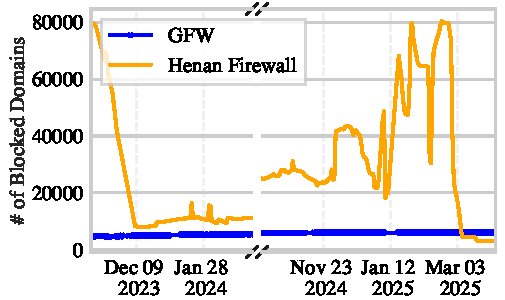
\includegraphics{figures/censored-domains-over-time-all.pdf}
  \caption{
    The numbers of domains
    blocked by the Henan Firewall and the GFW over time.
    We tested with a Tranco top one million domain list ID 5YZ7N,
    between November~5, 2023 and March~31, 2025,
    with a measurement gap between March~5 and October~7, 2024.
  }
  \label{fig:censored-domains-over-time}
\end{figure}

\parhead{Comparing the sizes of the blocklists over time.}
We monitored the changes to the blocklists of the Henan Firewall and the GFW over time.
\autoref{fig:censored-domains-over-time} shows
the total number of domains blocked by the Henan Firewall and the GFW.
The Henan Firewall has a blocklist that remains much larger than the GFW blocklist until March 4, 2025.

% see: ./data/README
% 1. The major cause of the “big drop” is the removal of at least 112 generic second-level domain blocking rules (e.g. *.com.au, *.net.br, *.gov.co).
% com.au,2023-11-22,100%,0%,5334,45,"Removal of com.au, Drop from 100% to 0%, 5334 to 45"
% 2. The first spike on Jan. 11 and Jan. 12 was mostly because of the addition and removal of *.com.au:
% com.au,2024-01-11,0%,99%,44,5331,"Addition of com.au, Jump from 0% to 99%, 44 to 5331"
% com.au,2024-01-12,99%,0%,5331,44,"Removal of com.au, Drop from 99% to 0%, 5331 to 44"
% 3. The second spike on Feb. 1 was mostly becaues of the addition of *.com.au. The down on Feb. 2 is because of removal of *.com.au.
% com.au,2024-02-01,0%,100%,27,5334,"Addition of com.au, Jump from 0% to 100%, 27 to 5334"
% com.au,2024-02-03,100%,0%,5334,26,"Removal of com.au, Drop from 100% to 0%, 5334 to 26"

The Henan Firewall frequently added and removed
generic second-level domain blocking rules (e.g. *.com.au, *.net.br, *.gov.co),
causing dramatic changes in the number of blocked domains.
For example,
~\autoref{fig:censored-domains-over-time} shows
a large consistent drop in the number of domains being blocked by the Henan Firewall,
between November 10 and December 8, 2023.
This drop was mostly due to the removal of at least 112 generic second-level domain blocking rules.
In particular,
the removal of the blocking rule *.com.au itself
contributed to the unblocking of more than five thousands domains on November 22, 2023.

\begin{table}[t]
  \caption{Top ten TLDs censored by the GFW and the Henan Firewall over a period of three months.
  The Henan Firewall blocked more country code top-level domain (ccTLDs) than the GFW.}
  \small
  \centering
  \begin{tabular}{rr|rr}
    \toprule
    \multicolumn{2}{c|}{\textbf{GFW}} & \multicolumn{2}{c}{\textbf{Henan}} \\ %\hline
    \textbf{TLD} & \textbf{Blocklist \%} & \textbf{TLD} & \textbf{Blocklist \%} \\
    \midrule
  %.com & 45.84\% & .com & 37.40\% \\ %\hline
  %.org & 6.17\% & .au & 11.43\% \\   %\hline
  %.net & 5.59\% & .za & 4.63\% \\    %\hline
  %.jp & 2.36\% & .net & 4.45\% \\    %\hline
  %.cc & 2.13\% & .uk & 4.11\% \\     %\hline
  %.de & 1.73\% & .org & 4.00\% \\    %\hline
  %.xyz & 1.72\% & .in & 2.87\% \\    %\hline
  %.in & 1.65\% & .jp & 2.35\% \\     %\hline
  %.tw & 1.50\% & .tw & 1.06\% \\     %\hline
  %.io & 1.31\% & .de & 1.02\% \\     %\hline

  .com & 45.8\% & .com & 37.4\% \\ %\hline
  .org & 6.1\% & .au & 11.4\% \\   %\hline
  .net & 5.6\% & .za & 4.6\% \\    %\hline
  .jp & 2.4\% & .net & 4.5\% \\    %\hline
  .cc & 2.1\% & .uk & 4.1\% \\     %\hline
  .de & 1.7\% & .org & 4.0\% \\    %\hline
  .xyz & 1.7\% & .in & 2.9\% \\    %\hline
  .in & 1.7\% & .jp & 2.4\% \\     %\hline
  .tw & 1.5\% & .tw & 1.1\% \\     %\hline
  .io & 1.3\% & .de & 1.0\% \\     %\hline


    \bottomrule

  \end{tabular}
  \label{table:tlds}
  \end{table}

We observe that the blocklist used by
the Henan Firewall also targets websites that are related to state or city
governance from other countries. For instance, a majority of state government
websites from the United States such as \textit{texas.gov, seattle.gov,
alabama.gov, nc.gov} are all blocked in Henan but not by the GFW. Compared to
the 83 \textit{*.gov*} domains that are seen in the GFW blocklist, we found 1002
\textit{*.gov*} domains blocked by the Henan Firewall,
showing an inclination to block anything that exhibits governance data or news from around the world. In
fact, we noticed a trend in the Henan Firewall to target country code top-level
domains (ccTLDs) more than the GFW as can be seen in~\autoref{table:tlds}.
Some of these blocks were widespread:
In 2024,
Henan blocked all 5,334 \textit{*.com.au}
domains we tested on Jan~19 and Feb~1--2,
all 2,075 \textit{*.co.za} domains
Feb~15--Mar~4,
and all 1,547 \textit{*.org.uk} domains Feb~8--Mar~4.
These may be instances of overblocking,
where the firewall contains an overly broad rule.
It is unclear to us why the Henan Firewall would repetitively block and unblock
these country code second level domains.

%The Henan Firewall blocklist
%comprised of 11.43\% \textit{.au} domains and 4.63\% of \textit{.za} domains.
%This shows that the Henan Firewall is more inclined to block ccTLDs compared to
%the GFW. \\

% Moreover, it was also interesting to see that domain names containing the word data were particularly targeted by the Henan Firewall. Websites such as \textit{worlddata.info}, \textit{civildatas.com}, and \textit{doctorsdata.com} were blocked in Henan but not by the GFW. This implies that the word 'data' is indeed a keyword being filtered for domain names by the Henan Firewall.

\parhead{Henan Firewall's blocklist is more volatile than the GFW's.}
%
\begin{figure}[t]
  \centering
  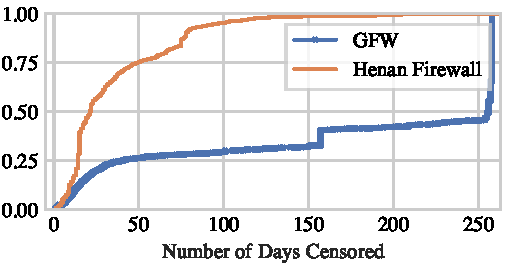
\includegraphics{figures/cdf-censored-duration-both.pdf}
  \caption{
    The censorship duration of all domains (ever) blocked by the GFW
    and the Henan Firewall between November~5, 2023 and March~31, 2025,
    with a measurement gap between March~5 and October~7, 2024.
    Compared to the GFW,
    the Henan Firewall has a more volatile blocking policy,
    with a larger proportion of domains being blocked for a shorter duration.
  }
  \label{fig:censorship-duration}
\end{figure}
%
% more analysis in censorship-duration/README
%GFW: mean=173.8, median=256.0, std=103.9
%Henan Firewall: mean=35.7, median=21.0, std=34.3
As shown in~\autoref{fig:censorship-duration},
the Henan Firewall has more volatile blocking policy than the GFW's blocklist.
While 75\% of blocked domains were censored for fewer than 51 days by the Henan Firewall,
more than 50\% of the domains ever censored by the GFW were blocked during the entire measurement period (256 days).
Domains blocked by the GFW had longer censorship durations (mean: 173.8 days; median: 256 days)
compared to those blocked by the Henan Firewall (mean: 35.7 days; median: 21 days).

As mentioned above,
this volatile blocking policy of the Henan Firewall is also mostly
due to the frequent addition and removal of generic second-level domain blocking rules.
For example,
\autoref{fig:censored-domains-over-time} shows
two spikes in the number of domains blocked by the Henan Firewall
between January 11 and January 12, 2024,
as well as between February 1 and February 3, 2024.
They are mostly due to the addition and removal of the blocking rule *.com.au.
It worth noting that even when the rule *.com.au was removed,
for example on January 12 and February 3, 2024,
the Henan Firewall still blocked 44 and 26 domains ended with .com.au, respectively.
This observation suggests that the blocking rule can be finer grained than the second-level domain.


\begin{figure}[t]
  \centering
  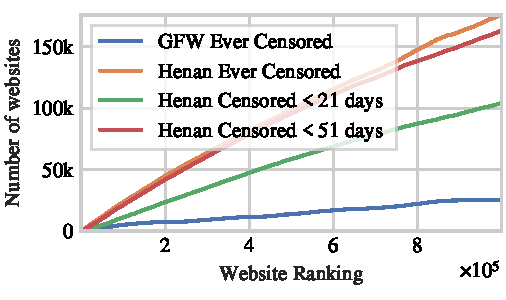
\includegraphics[width=\linewidth]{figures/cdf-ranking.pdf}
  \caption{
  Cumulative distribution of the domains blocked by the GFW and the Henan Firewall
  in the Tranco top one~million list 5YZ7N.
  The data is collected between November~5, 2023 to March~31, 2025,
  with a measurement gap between March~5 and October~7, 2024.
  }
  \label{fig:cdf-ranking}
\end{figure}

\parhead{Do the two firewalls target similar websites?}
\autoref{fig:cdf-ranking} shows the cumulative distribution of the domains blocked by the GFW
and by the Henan regional censorship devices among the top one million Tranco domains over
our measurement period of nine months.
% The data is aggregated over more than nine months from November~5, 2023 to March~31, 2025 with
% a measurement gap between March~5 and October~7, 2024.

For the GFW, we classify a domain as blocked if it was blocked at least once
during our measurement period. Due to the volatility of the Henan Firewall's blocklist,
we categorize domains into three classes: those that were ever blocked,
those blocked for less than 21 days, and those blocked for less than 51 days.
We selected these thresholds based on our observation of average blocking durations
for both firewalls, as shown in~\autoref{fig:censorship-duration}.

During our measurement period, we cumulatively observed 25,441 domains censored by the GFW,
while 175,925 domains were blocked at least once by the Henan Firewall.
Of the domains censored by the Henan Firewall, our analysis identified 104,100 domains
with blocking periods under 21 days, while 163,083 domains experienced blocking durations shorter than 51 days.

Looking at the cumulative distribution and the ranking of the domains,
we found that the most popular domains were more likely to be blocked by both the GFW and the Henan Firewall.
The Henan Firewall is more homogeneous in blocking domains in terms of their popularity whereas the GFW's blocklist exhibits a more heterogeneous distribution.
While the GFW firewall targets the more popular websites,
as can be seen from the graph,
the Henan Firewall targets the websites more uniformly.
However, the sizes of the two blocklists provide a stark contrast between the two firewalls.

\parhead{Overlap between the two blocklists.}
% $ head zones_sni_censorship_guangzhou-2_ts_0_2023-12-26_04-00-02.csv.1
% 1703534402183,000000okwegjjxzqe1g2udb9z6ognw.com.,TLS,EOF,
% Mon Dec 25 2023 20:00:02 GMT+0000
% Thu Feb 22 2024 05:53:45 GMT+0000
To understand the sizes and overlap of the two blocklists,
we perform a long-running experiment to test 227~million domains on a weekly basis,
between December~26, 2023 and March~31, 2025.
\autoref{fig:venn-diagram-acc}
shows the accumulated blocklists of the GFW and the Henan Firewall.
During the experiment,
the Henan Firewall blocked 4,196,532 domains---more than five times the 741,542 domains ever blocked by the GFW.
There are 479,247 domains blocked by both firewalls.
The Jaccard index between the two blocklists is approximately 0.0885,
indicating they share under 9\% similarity and are therefore largely independent yet complementary in their coverage.
% $J = \frac{|H \cap G|}{|H \cup G|} \approx 0.0885$, where $J$ is the Jaccard index, $H$ is the set of domains blocked by the Henan Firewall, and $G$ is the set of domains blocked by the Great Firewall (GFW).


\begin{figure}[t]
  \includegraphics[width=\linewidth]{figures/venn-diagram-accumulated.pdf}
  \caption{
    Venn diagram of the cumulative domains ever blocked by the GFW and the Henan Firewall.
    We conducted weekly testing of 227~million domains
    between
    December~26,~2023
    and
    March~31,~2025 (with a measurment gap between March~5 and October~7, 2024).
    The Henan blocklist is more than five times the size of the GFW blocklist.
    }
    \label{fig:venn-diagram-acc}
\end{figure}


\parhead{Categorizing the blocked domains.}
%To answer the question of what type of content is being blocked by the Henan Firewall compared to GFW,
we used the \textit{whoisxmlapi.com}~\cite{WebsiteC13:online} website categorization service
to classify the blocklists obtained for each firewall between November 21, 2023, and January 15, 2024.
We acknowledge that not all domains could be categorized, as some were inactive or did not host content.
\autoref{tab:categories} shows the top ten categories of censored domains for each firewall.

\begin{table}[h!]
  \centering
  \caption{
    The top categories of domains blocked by the Henan Firewall and the GFW
    among the top one million Tranco domains.
    Categories not in the top ten of each firewall are marked as ``-''.
    }
  \begin{tabular}{lS[table-format=4.0]S[table-format=3.1]S[table-format=3.0]S[table-format=3.1]}
      \toprule
      \textbf{Category} & \multicolumn{2}{c}{\textbf{Henan}} & \multicolumn{2}{c}{\textbf{GFW}} \\
      \cmidrule(lr){2-3} \cmidrule(lr){4-5}
      & \textbf{Count} & \textbf{Portion (\%)} & \textbf{Count} & \textbf{Portion (\%)} \\
      \midrule
      Business           & 4861 & 26.9 & 1183 & 15.3 \\
      Computer     & 2517 & 13.9 & 642  & 8.3  \\
      Pornography          & 2394 & 13.2 & 2207 & 28.6 \\
      Gambling                      & 1276 & 7.1  & {--} & {--} \\
      Society                       & 1265 & 7.0  & 459  & 5.9  \\
      Shopping                      & 1261 & 7.0  & 288  & 3.7  \\
      Travel                        & 1230 & 6.8  & {--} & {--} \\
      Entertainment         & 1134 & 6.3  & 548  & 7.1  \\
      Education       & 1104 & 6.1  & {--} & {--} \\
      Uncategorized                 & 1057 & 5.8  & 395  & 5.1  \\
      News                 & {--} & {--} & 1378 & 17.9 \\
      Personal Sites       & {--} & {--} & 313  & 4.1  \\
      Streaming Media               & {--} & {--} & 305  & 4.0  \\
      \bottomrule
  \end{tabular}
  \label{tab:categories}
\end{table}

An interesting point that we note here is that the Henan Firewall targets
Business, Economy, Computer and Internet Information domains more than the GFW.
More than 35\% of the total domains appearing on the blocklist of the Henan
Firewall were from these two categories.
To find the reason behind the focus on these categories,
we hypothesize that the province of Henan has been a center of a lot of financial
controversies, with the most prominent being the mass protests in 2022 that were a
result of a financial scandal involving local lenders~\cite{Security88:online}.
Given the financial scandals targeting state-controlled financial institutions, it is very
probable that the state wants to limit access to information that is relevant
to the economy of the area. On the other side, it could be a part of the
national policy to censor critics of the country's business and economic policies.

The GFW on the other hand, targets more of the news and media, as well as adult content domains.
This is in line with the long-standing understanding of the GFW that
it aims to limit more of the news, morally sensitive and politically sensitive content.


\subsection{Identifying the Blocking Rules}
Another way to view how each of the firewalls configures filter rules is to infer
likely regular expressions used for blocklist matching.
As noted by Anonymous et~al.~\cite[\S 6]{Anonymous2014a}
and Hoang et~al.~\cite[\S 4.1]{Hoang2021a} in their study of the GFW's DNS censorship,
the GFW blocks domains using rules that may target
second-level domains, top-level domains, and/or subdomains. They developed a
methodology to encompass the blocking rules applied by the GFW. We used a
similar methodology based on the permutations listed
in~\autoref{tab:domain_patterns} to infer blocking rules for both the Henan
Firewall and GFW. We note that our inferred regular expressions may not fully
reflect the rules employed by the censor, as our permutations can miss
regular expressions based on second-level domains or more complex regular
expressions such as \texttt{*.gov*} that we observe the Henan Firewall blocking.
Nonetheless, our inferred rules allow us to identify structural differences in
the blocklists of the Henan Firewall compared to the GFW.

\begin{table}[t]
  \centering
  \small
  \caption{Permutations used to test the blocking rules of the Henan Firewall and the GFW.
  The placeholder \texttt{\{str\}} represents strings that,
  alone or combined with others,
  should not trigger censorship.
  In this work,
  we used the string \texttt{ZZZZ}.
  }
  \begin{tabular}{ll ll}
    \toprule
    \textbf{Test} & \textbf{Pattern} & \textbf{Test} & \textbf{Pattern} \\
    \midrule
    Test 0 & \{str\}domain\{str\} & Test 5  & \{str\}domain \\
    Test 1 & domain & Test 6 & \{str\}.domain.\{str\} \\
    Test 2 & domain.\{str\} & Test 7 & \{str\}.domain\{str\} \\
    Test 3 & domain\{str\} & Test 8 & \{str\}domain.\{str\} \\
    Test 4 & \{str\}.domain & & \\
    \bottomrule
  \end{tabular}
  \label{tab:domain_patterns}
\end{table}

As shown in~\autoref{tab:domain_patterns},
we generated nine permutations for each censored domain
identified in our daily measurement experiment (\autoref{sec:blocklists}),
by prepending and/or appending a fixed string to the domain name.
This methodology was used by
Anonymous~et~al.~\cite[\S 6]{Anonymous2014a} in 2014
and Hoang~et~al.~\cite[\S 4.1]{Hoang2021a} in 2021.
We chose the pattern string \texttt{ZZZZ} to construct each permutation in this work.
We then sent ClientHellos with SNI containing each permutation independently to our sink servers
and recorded the results for each testing.
This experiment was conducted four times daily during our measurement period.

% cat gfw-rule-count.tsv
% token	count	percentage
% 1,4	163355	85.07
% 1	17764	9.25
% 1,2,3,4,6,7	7272	3.79
% 1,4,5	2483	1.29
% 1,2,3,4,5,6,7,8,0	647	0.34
% 4	429	0.22
% 1,2,3	36	0.02
% 1,2,4,6,7	6	0.00
% 1,3,4,6,7	5	0.00
% 1,2,3,4,6	3	0.00
% 1,3,4,6	2	0.00
% 1,4,6	2	0.00
% 1,2,3,6,7	2	0.00
% 1,2,3,4,7	2	0.00
% 1,2,4,6	1	0.00
% 1,4,6,7	1	0.00
% 3	1	0.00
% 3,7	1	0.00
% 1,2,4,7	1	0.00
% 2,3,4,6,7	1	0.00
% 1,2,4	1	0.00
% 4,6	1	0.00
% 3,4,6,7	1	0.00
% 1,2,3,4	1	0.00

% cat henan-rule-count.tsv
% token	count	percentage
% 1,4	248770	64.06
% 1,4,5	139575	35.94
% 4	4	0.00
% 1	3	0.00
% 1,5	2	0.00

% Sanity checked on: https://regex101.com
% ZZZZkeywordZZZZ
% keyword
% keyword.ZZZZ
% keywordZZZZ
% ZZZZ.keyword
% ZZZZkeyword
% ZZZZ.keyword.ZZZZ
% ZZZZ.keywordZZZZ
% ZZZZkeyword.ZZZZ

\begin{table}[t]
  \centering
  \caption{
  We infer the regex equivalents of blocking rules employed by
  the GFW and the Henan Firewall.
  In total, the GFW and the Henan Firewall employ 24 and 5 unique regex patterns, respectively.
  The table only shows the regex patterns that have more than ten occurrences for the GFW.
  }
  {\setlength{\tabcolsep}{5pt} % Reduce inter-column spacing
  \begin{tabular}{@{}llrrrr@{}}
    \toprule
    \textbf{Inferred Regex} & \textbf{Tests Hit} & \multicolumn{4}{c}{\textbf{Rule Count (Portion)}} \\
    \cmidrule(lr){3-6}
                           &                  & \multicolumn{2}{c}{\textbf{GFW}}   & \multicolumn{2}{c}{\textbf{Henan}}   \\
    \midrule
    \verb|^(.*\.)?keyword$|   &       1\&4             & 163,355 & 85\%  & 248,770 & 64\%  \\
    \verb|^keyword$|          &       1                & 17,764 & 9.3\%  & 3 & 0.0\%       \\
    \verb|^(.*\.)?keyword|    &       1--4\&6\&7       & 7,272 & 3.8\%   & --  & --            \\
    \verb|keyword$|           &       1\&4\&5          & 2,483 & 1.3\%   & 139,575 & 36\%  \\
    \verb|keyword|            &       0--8             & 647 & 0.3\%     & --  & --            \\
    \verb|\.keyword$|         &       4                & 429 & 0.2\%     & 4 & 0.0\%       \\
    \verb|^keyword|           &       1\&2\&3          & 36 & 0.0\%     & --  & --            \\
    \bottomrule
  \end{tabular}
  }
  \label{tab:regex}
\end{table}

% TODO: update the text.
As shown in~\autoref{tab:regex},
the most popular blocking regex pattern used by both the Henan Firewall and the GFW
was \verb|^(.*\.)?keyword$|.
This pattern meant to be used to block a domain and its subdomains.
The second most popular blocking regex pattern used by the GFW was \verb|^keyword$|,
which was used to only block the domain name itself, not its subdomains.
The third most popular blocking regex pattern used by the GFW was \verb|^(.*\.)?keyword|,
which was likely to be a mistake of not including the end anchor in the regex pattern.
Interestingly,
unlike the GFW, which sometimes employs regex patterns without end anchors,
the Henan Firewall always includes end anchors in its regex patterns.
This result could be because of a more carefully and consistently maintained blocklist,
or perhaps the censorship implementation itself enforces the use of end-anchored regex patterns to prevent potential mistakes made by human.


% \begin{figure}[t]
%   \centering
%   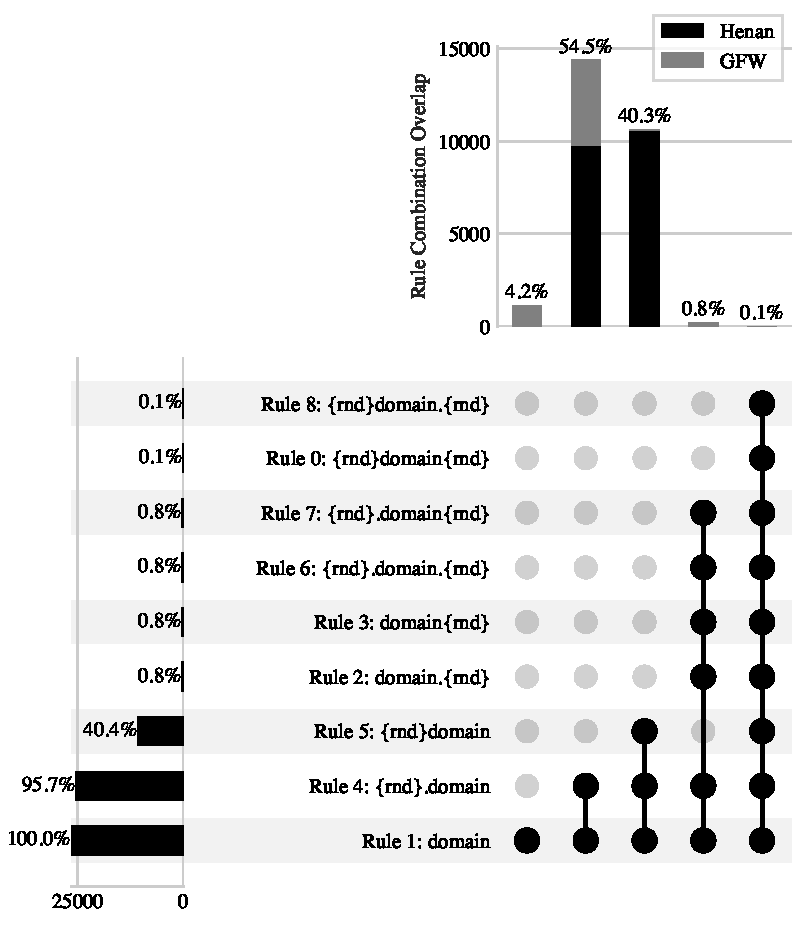
\includegraphics[]{figures/rule-extraction.pdf}
%   \caption{
%   Out of the top one million domains that were blocked,
%   we extracted the rules used to block them.
%   We found that rules 1 and 4 were the most frequently used in combination to block domains.
%   The combination of rules 1, 4, and 5 was the second most popular blocking pattern.
%   }
%   \label{fig:rule-extraction}
% \end{figure}


% python3 plot.py --gfw gfw-blacklist-categorized.csv --out "gfw-categorized.pdf" --no-show
% category,count,portion
% Adult and Pornography,2207,28.6
% News and Media,1378,17.9
% Business and Economy,1183,15.3
% Computer and Internet Info,642,8.3
% Entertainment and Arts,548,7.1
% Society,459,5.9
% Uncategorized,395,5.1
% Personal sites and Blogs,313,4.1
% Streaming Media,305,4.0
% Shopping,288,3.7

% python3 plot.py --henan henan-blacklist-categorized.csv --out "henan-categorized.pdf" --no-show
% category,count,portion
% Business and Economy,4861,26.9
% Computer and Internet Info,2517,13.9
% Adult and Pornography,2394,13.2
% Gambling,1276,7.1
% Society,1265,7.0
% Shopping,1261,7.0
% Travel,1230,6.8
% Entertainment and Arts,1134,6.3
% Educational Institutions,1104,6.1
% Uncategorized,1057,5.8

% python3 plot.py --henan overlap_categorized.csv --out "overlap-categorized.pdf" --no-show
% category,count,portion
% Adult and Pornography,779,37.2
% Business and Economy,352,16.8
% Computer and Internet Info,163,7.8
% Entertainment and Arts,145,6.9
% Uncategorized,145,6.9
% News and Media,117,5.6
% Society,106,5.1
% Gambling,101,4.8
% Shopping,94,4.5
% Travel,91,4.3

% \begin{figure}[t]
% \begin{subfigure}[]{\linewidth}
%     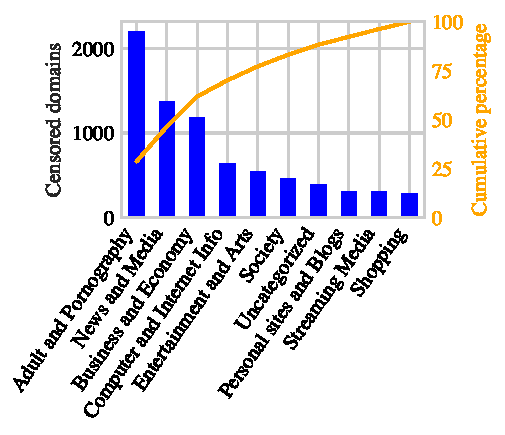
\includegraphics[width=\textwidth]{figures/gfw-categorized}
%     \caption{GFW}
%     \label{fig:first}
% \end{subfigure}
% % \hfill
% \begin{subfigure}[]{\linewidth}
%     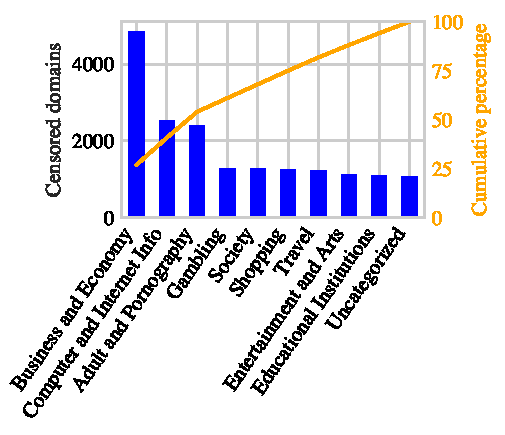
\includegraphics[width=\textwidth]{figures/henan-categorized}
%     \caption{Henan Firewall}
%     \label{fig:second}
% \end{subfigure}
% % \hfill

% \caption{Categorization of domains blocked by the GFW and the Henan Firewall among the top one million Tranco domains.}
% \label{fig:categories}
% \end{figure}



\section{Circumvention Strategies}
\label{sec:circumvention}

Based on the parsing logic flaws we identified in~\autoref{sec:parsing-logic},
as well as the injection behaviors and fingerprints we observed in~\autoref{sec:how-block},
we introduce simple but effective strategies to bypass the Henan Firewall.
All strategies require only changes from the client-side,
without cooperation from the server side,
making them easy to employ and adopt.
These strategies have already been implemented in various popular circumvention tools,
including but not limited to
Xray~\cite{Xray},
GoodbyeDPI~\cite{GoodbyeDPI},
and Shadowrocket~\cite{shadowrocket}.

\parhead{Enable any TCP option field.}
As detailed in~\autoref{sec:parsing-logic},
the Henan Firewall can only parse and block TCP packets with a 20-byte header.
% Enabled this on all packets via: tcp_layer = TCP(sport=RandShort(), dport=443, flags='PA', options=[('NOP', None)])
Enabling any TCP option on an operating system will result in
a TCP header longer than 20 bytes.
While this circumvention solution relies on the unusual implementations of the Henan Firewall,
it is nonetheless a feature that users or circumvention tools could easily employ to evade censorship.
For instance,
enabling TCP Timestamps (disabled by default on some version of the Windows) would
prevent the Henan Firewall from blocking connections~\cite{tsinbei_tcp_timestamps,net4people442}.

%We tested this by sending SYN packets with different TCP options set in the TCP handshake,
%including MSS, Window Scale, NOP, and Timestamps.
%We then sent a TLS ClientHello message containing a blocked domain name \texttt{011.com} as the SNI.
%We observed that,
%possibly due to its poor parsing logic,
%the Henan Firewall did not block the connection when any of these TCP options was set.
%%
%As an example,
%enabling TCP timestamp option field is an easy-to-apply circumvention strategy.
%The TCP Timestamp (TSval) is a 32-bit timestamp value attached to every non-RST TCP segment.
%It is a relative timestamp often to measure the round-trip time (RTT) of a TCP connection
%and the implementation of it varies across different operating systems.
%While Linux and MacOS machines have the TCP Timestamps option field enabled by default,
%Windows machines often have it disabled.
%Windows users can thus enable the TCP Timestamps option field to bypass the Henan Firewall.
%% While the exact reasoning for this strange behavior is difficult to understand,
%% it is nevertheless a circumvention strategy that could be used to bypass the Henan Firewall.

\parhead{Discard TCP \texttt{RST} packets with specific payload.}
As shown in~\autoref{sec:how-block},
the Henan Firewall injects a TCP \texttt{RST} packet with an unusual 10-byte payload
\begin{bytebox}\x{01}\x{02}\x{03}\x{04}\x{05}\x{06}\x{07}\x{08}\x{09}\x{00}\end{bytebox}.
Its uniquesness allows the client drop only the \texttt{RST} packets injected by the Henan Firewall,
while keeping the \texttt{RST} packets sent by the server.
Typically,
dropping TCP \texttt{RST} packets sent to the client is not enough to evade TCP \texttt{RST} censorship by the GFW,
as the GFW also injects \texttt{RST} packets to the server.
However, as explained in~\autoref{sec:how-block},
the Henan Firewall only injects \texttt{RST} packets to the client,
and thus dropping the \texttt{RST} packets sent to the client is sufficient to evade censorship.
This circumvention strategy can be easily applied via \texttt{iptables} rules,
similar to the ones introduced by Clayton et~al.~\cite[\S 5]{Clayton2006a}.
%Additionally,
%should the censor change the payload pattern in the future,
%one can apply a more general rule to block all \texttt{RST} packets with a payload,
%as the vast majority of \texttt{RST} packets do not contain a payload.


\parhead{Segment or fragment TLS ClientHello into multiple packets.}
As expalined in~\autoref{sec:parsing-logic},
the Henan Firewall does not perform TCP reassembly,
and neither the Henan Firewall nor the GFW performs TLS reassembly~\cite{Niere2023a}.
Thus, clients can segment TCP packets or
fragment TLS ClientHello messages over multiple TLS records to evade the Henan firewall~\cite{Niere2023a}.
As long as the TCP packets carrying the beginning part of ClientHello messages
does not contain a complete SNI extension,
one can bypass the Henan Firewall.
Performing this fragmentation may require TLS libraries such as uTLS~\cite{Frolov2019a} that
provide fine-grained control over the messages sent, or purposely built
circumvention tools like DPYProxy~\cite{GoodbyeDPI} that can fragment records
made by a browser.
Popular circumvention tools such as
Xray~\cite{Xray} and Shadowrocket~\cite{shadowrocket}
have also implemented this TCP segmentation strategy~\cite{xraypullrrequest}.



%and thus,
%it is possible to bypass it by splitting the TCP payload into multiple TCP segments.
%In particular,
%one can bypass the Henan Firewall,
%as long as the first TCP segment does not contain a complete SNI extension.
%Tools
%
%\parhead{Fragment TLS ClientHello into multiple TLS records.}
%We find that neither the Henan Firewall nor the GFW perform TLS reassembly.
%It is thus possible to bypass both of their censorship
%by fragmenting TLS ClientHello messages over multiple TLS records.
%% TODO: redo the experiment and check-in the scripts to the repo.
%In particular,
%as long as the first TLS record does not contain a complete SNI extension,
%even if the SNI extension in the other TLS record is still within the same TCP packet,
%one can bypass the Henan Firewall.
%

\section{Ethics}
\label{sec:ethics}

Censorship measurement studies,
especially in authoritarian regimes,
require careful ethical considerations
and continuous evaluation of the potential risks involved
throughout the entire research process.
%
In this work,
we conducted all of our censorship measurements from machines we controlled,
with network traffic generated automatically by our programs.
This approach is a common practice in censorship measurement studies
to mitigate the risk of overwhelming other hosts on the Internet
and imposing any risks on users~\cite{Wu2023a, Alice2020a, Hoang2024a, Hoang2021a, Anonymous2020a}.
When analyzing the real-world traffic on the university network tap,
we only collected the TCP header length fields of the packets
without capturing any human identifiable or sensitive information.
Since IRB approval is thus not applicable for this study (as it does not involve human subjects),
we followed the ethical guidelines outlined in the Menlo Report~\cite{menlo-report}.
Our research team also consulted experts with a deep understanding of
Chinese censorship and its legal concerns.
% for the choice of vantage points
% and the design of our measurement experiments.
% C.3.1 Identification of Potential Benefits and Harms
Below,
we discuss the potential risks we identified and the steps we took to mitigate them~\cite[\S C.3.2]{menlo-report}.

\parhead{Traffic analysis.}
%
To evaluate the effectiveness of the Henan Firewall,
we measured the TCP header length fields of all TCP packets on the university network tap.
The use of this network tap was approved by the university's privacy and security office.
We also worked closely with the campus networking and security teams who has experience managing similar projects.
This approval and collaboration ensured that
we followed standard security procedures,
complied with network use policy,
respected user privacy,
and minimized the network’s attack surface.
Additionally, we designed the tap to only receive a copy of traffic,
ensuring no impact on network users in case of system failure.

We designed our experiment to avoid collecting any potentially sensitive information,
such as IP addresses,
which could be linked to individuals.
Specifically, we only collected the 4-bit Data Offset fields from all TCP headers in an aggregated manner.
We never inspected or logged any raw traffic data.
%
We practiced the principle of least privilege
by restricting access to the network tap to a limited,
authorized subset of our team.


\parhead{Vantage points.}
%
Obtaining vantage points within censored areas has become increasingly challenging.
However,
two key research questions we aim to answer require
diverse vantage point coverage in China:
1) Is the Henan Firewall also deployed in other provinces in China?
2) Do other provinces deploy their regional censorship apparatus as well?
% C.3.2 Balancing Risks and Benefits
We took extra care to find the right balance
between finding as diverse vantage points as possible
and the potential risks it carries~\cite[\S C.3.2]{menlo-report}.
For example,
while using residential vantage points would have allowed us to observe censorship
in China from more network locations,
we decided not to use them due to the potential risks to the uninformed users~\cite{Mi2019-resident-evil}.

We also explored the possibility of measuring the Henan Firewall remotely from outside of the province or China,
which will further reduce the risks of initiating connections from within the region;
however, as introduce in~\autoref{sec:what-targeted},
the Henan Firewall could not be triggered that way.

We thus,
following the rationale and common practices outlined in prior work~\cite{Wu2023a,Alice2020a},
strategically selected vantage points provided by large commercial cloud providers
to mitigate potential legal risks for individuals.
We registered our VPS accounts with the accurate identity
and contact information of one of our researchers who is
neither a citizen nor a resident of China.
Throughout our research,
we received no complaints from the providers.
To avoid the possibility of getting other cloud users' resources blocked by the censor,
we assigned dedicated IP addresses to each of our machines.

\parhead{Probing rate and design.}
%
To avoid overwhelming our vantage points and the network paths our probes traversed,
we restricted the transmission speed directed to our sink servers.
For experiments in~\autoref{sec:detection} and ~\autoref{sec:characterization},
we limited the probing rate
to no more than one connection per second;
for experiments in~\autoref{sec:blocklists},
we set a hard limit on each client to send no more than 1 Mbps of traffic.
%
While the risks and potential harms of our probes being logged by the censor is minimal,
we also designed our experiments with plausible deniability in mind.
That is,
since our sink servers never replied with any ServerHello messages or HTTP responses,
and no full TLS or HTTP connections were ever established,
our measurement behaviors do not resemble users accessing censored websites.


\section{Conclusion}

In this paper,
we expose and document an alarming sign in China's Internet censorship strategy:
our measurements from seven different cities and provinces in China
reveal a new regional firewall in Henan province.
This Henan Firewall conducts HTTP Host-based and TLS SNI-based censorship
for traffic going out of the province.
It exhibits distinct characteristics compared to the GFW,
including unique packet injection behaviors and fingerprints,
different logic in tracking, parsing, and blocking connections,
a once ten-times larger and more dynamic blocklist,
and closer network location to the client.
This localized censorship suggests a departure from China's centralized
censorship apparatus, enabling local authorities to exert a greater degree of
control within their respective regions.
We propose simple but effective circumvention techniques to get around
this emerging system in Henan,
which have been implemented in vairous popular circumvention tools.
We hope our study sounds the alarm to the
broader censorship research community to be aware of and further study
emerging regional censorship in China, and elsewhere.


% conference papers do not normally have an appendix

\section*{Availability}
To encourage future research and promote transparency and reproducibility,
we have made the code, anonymized data, and constantly updated blocklists available.
For improved accessibility,
this paper is also available in HTML format in both English and Chinese.
The project homepage is at: \url{https://gfw.report/publications/sp25/en}.


% use section* for acknowledgement
\section*{Acknowledgments}
We thank our shepherd and other anonymous reviewers for their valuable comments and feedback.
We also thank the brave users in China for immediately reporting and actively studying the blocking incidents,
including, but not limited to,
5e2t, Hsukqi, ThEWiZaRd0fBsoD, louiesun, and lemon99ee.
We are grateful to
ValdikSS,
radioactiveAHM,
RPRX,
Fangliding,
GFW-knocker,
sambali9,
rrouzbeh,
nekohasekai,
znlihk,
the V2Ray developers,
the Hysteria developers,
the Shadowrocket developers,
and many other developers for
their helpful discussions
and/or for
integrating TCP segmentation and/or TLS fragmentation features into their respective circumvention tools.
We also thank
Jackson Sippe,
Jade Sheffey,
Paul Flammarion,
the Stanford Empirical Security Research Group,
the Stanford University security and networking teams,
and many others who prefer to remain anonymous
for their helpful discussions and support.
We thank Net4People BBS,
NTC Party forum,
Xray community, V2Ray community, and sing-box community
for providing online space for censorship discussions.
We are grateful to David Fifield for providing feedback, support, and guidance throughout the entire project.

The work was supported in part by the National Science Foundation (NSF) under grant numbers
CNS-2145783, CNS-2319080, and CNS-2333965,
by a Sloan Research Fellowship,
and by the
Young Faculty Award program of the Defense Advanced Research Projects
Agency (DARPA) under the grant DARPA-RA-21-03-09-YFA9-FP-003.
The views, opinions, and/or findings expressed are those of the
authors and should not be interpreted as representing the official
views or policies of the Department of Defense or the U.S. Government.

% The authors would like to thank...

\balance
\bibliographystyle{IEEEtran}
\bibliography{censor,main}

% \appendix

\newpage % The Meta-Review should at least start on a new column

% Use \appendices and not \appendix due to IEEEtran.cls quirks
\appendices % if not used earlier

\section{Meta-Review}

The following meta-review was prepared by the program committee for the 2025
IEEE Symposium on Security and Privacy (S\&P) as part of the review process as
detailed in the call for papers.

\subsection{Summary}

This paper empirically confirms anecdotal evidence that the Henan province in China had started to deploy regional censorship mechanisms, purposely more stringent than those employed by the great firewall itself. The paper delivers a comprehensive analysis of censorship carried out by the Henan Firewall, both on in/out and out/in directions, shedding light on its functioning, blocking policies, and residual censorship mechanisms. In addition, the paper inspects whether similar regional censorship is occurring in other Chinese provinces, finding no evidence of additional interference beyond that of the great firewall.

\subsection{Scientific Contributions}


\begin{itemize}
\item Independent Confirmation of Important Results with Limited Prior Research
\item Provides a Valuable Step Forward in an Established Fieldtext
\end{itemize}

\subsection{Reasons for Acceptance}
\begin{enumerate}
\item This paper provides an independent confirmation of important results with limited prior research.  The paper builds a measurement apparatus to confirm (and expand on the information provided by) anecdotal reports of regional censorship within the Henan province in China. Besides providing a systematic understanding of the existence and blocking behavior of this new type of regional censorship, the paper also independently confirms the asymmetry in blocking behavior of the great firewall.
\item The paper provides a valuable step forward in an established field by applying different known methodologies to exhaustively study a new phenomenon of censorship in a part of China. The measurements carried out in the presented study are sound and rely on true-and-tested measurement methodologies, providing insights into a form of censorship that had not been further analyzed.
\end{enumerate}

% \subsection{Noteworthy Concerns} % Exclude if your meta-review does not have noteworthy concerns
% \begin{enumerate} % Enumerate environment is not necessary if there is only one
% \end{enumerate}

% \section{Response to the Meta-Review} % Optional

% Less than 500 words response to the meta-review. The response to the
% meta-review is optional. Provide a response if you disagree with the
% meta-review. Shepherds will only deny responses to meta-reviews if they are too
% long or are abusive / inappropriate.


% that's all folks
\end{document}
